\documentclass[preprint, 3p,
authoryear]{elsarticle} %review=doublespace preprint=single 5p=2 column
%%% Begin My package additions %%%%%%%%%%%%%%%%%%%

\usepackage[hyphens]{url}

  \journal{An awesome journal} % Sets Journal name

\usepackage{graphicx}
%%%%%%%%%%%%%%%% end my additions to header

\usepackage[T1]{fontenc}
\usepackage{lmodern}
\usepackage{amssymb,amsmath}
% TODO: Currently lineno needs to be loaded after amsmath because of conflict
% https://github.com/latex-lineno/lineno/issues/5
\usepackage{lineno} % add
\usepackage{ifxetex,ifluatex}
\usepackage{fixltx2e} % provides \textsubscript
% use upquote if available, for straight quotes in verbatim environments
\IfFileExists{upquote.sty}{\usepackage{upquote}}{}
\ifnum 0\ifxetex 1\fi\ifluatex 1\fi=0 % if pdftex
  \usepackage[utf8]{inputenc}
\else % if luatex or xelatex
  \usepackage{fontspec}
  \ifxetex
    \usepackage{xltxtra,xunicode}
  \fi
  \defaultfontfeatures{Mapping=tex-text,Scale=MatchLowercase}
  \newcommand{\euro}{€}
\fi
% use microtype if available
\IfFileExists{microtype.sty}{\usepackage{microtype}}{}

\ifxetex
  \usepackage[setpagesize=false, % page size defined by xetex
              unicode=false, % unicode breaks when used with xetex
              xetex]{hyperref}
\else
  \usepackage[unicode=true]{hyperref}
\fi
\hypersetup{breaklinks=true,
            bookmarks=true,
            pdfauthor={},
            pdftitle={A historical analysis of the evolution of active travel behaviour in Canada},
            colorlinks=false,
            urlcolor=blue,
            linkcolor=magenta,
            pdfborder={0 0 0}}

\setcounter{secnumdepth}{5}
% Pandoc toggle for numbering sections (defaults to be off)


% tightlist command for lists without linebreak
\providecommand{\tightlist}{%
  \setlength{\itemsep}{0pt}\setlength{\parskip}{0pt}}


% Pandoc citation processing
%From Pandoc 3.1.8
% definitions for citeproc citations
\NewDocumentCommand\citeproctext{}{}
\NewDocumentCommand\citeproc{mm}{%
  \begingroup\def\citeproctext{#2}\cite{#1}\endgroup}
\makeatletter
 % allow citations to break across lines
 \let\@cite@ofmt\@firstofone
 % avoid brackets around text for \cite:
 \def\@biblabel#1{}
 \def\@cite#1#2{{#1\if@tempswa , #2\fi}}
\makeatother
\newlength{\cslhangindent}
\setlength{\cslhangindent}{1.5em}
\newlength{\csllabelwidth}
\setlength{\csllabelwidth}{3em}
\newenvironment{CSLReferences}[2] % #1 hanging-indent, #2 entry-spacing
 {\begin{list}{}{%
  \setlength{\itemindent}{0pt}
  \setlength{\leftmargin}{0pt}
  \setlength{\parsep}{0pt}
  % turn on hanging indent if param 1 is 1
  \ifodd #1
   \setlength{\leftmargin}{\cslhangindent}
   \setlength{\itemindent}{-1\cslhangindent}
  \fi
  % set entry spacing
  \setlength{\itemsep}{#2\baselineskip}}}
 {\end{list}}
\usepackage{calc}
\newcommand{\CSLBlock}[1]{#1\hfill\break}
\newcommand{\CSLLeftMargin}[1]{\parbox[t]{\csllabelwidth}{#1}}
\newcommand{\CSLRightInline}[1]{\parbox[t]{\linewidth - \csllabelwidth}{#1}\break}
\newcommand{\CSLIndent}[1]{\hspace{\cslhangindent}#1}


\usepackage{booktabs}
\usepackage{longtable}
\usepackage{array}
\usepackage{multirow}
\usepackage{wrapfig}
\usepackage{float}
\usepackage{colortbl}
\usepackage{pdflscape}
\usepackage{tabu}
\usepackage{threeparttable}
\usepackage{threeparttablex}
\usepackage[normalem]{ulem}
\usepackage{makecell}
\usepackage{xcolor}



\begin{document}


\begin{frontmatter}

  \title{A historical analysis of the evolution of active travel
behaviour in Canada}
    \author[Some Institute of Technology]{Alice Anonymous%
  \corref{cor1}%
  \fnref{1}}
   \ead{alice@example.com} 
    \author[Some Institute of Technology]{Bob Security%
  %
  \fnref{1}}
   \ead{bob@example.com} 
    \author[Some Institute of Technology]{Cat Memes%
  %
  }
   \ead{cat@example.com} 
      \affiliation[Some Institute of Technology]{
    organization={Big Wig University},addressline={1 main
street},city={Gotham},postcode={123456},state={State},country={United
States},}
    \cortext[cor1]{Corresponding author}
    \fntext[1]{These authors contributed equally to this work.}
  
  \begin{abstract}
  Impedance functions are used to represent travel behaviour due to
  their potential to capture traveler responses to geographic distance
  between origins and destinations. Focusing our analysis on active
  transportation modes in Canadian metropolitan regions, this study has
  as objectives to provide an historical overview of active mobility in
  terms of main origins, destinations and travel time of walking and
  cycling trips, and to identify appropriate impedance functions for
  active transportation modes considering a wide range of destinations
  and time periods. To achieve these objectives, this paper analyzed
  more than cases of 12,000 active transportation episodes, that
  represented more than 12 million episodes, from the Canadian General
  Social Survey (GSS) from 1992 to 2015. This study confirmed that for
  walking trips, typical travel times remained constant at 10 minutes
  since 2005, while for cycling trips, typical travel times fluctuated,
  declining from 20 minutes in 1992 to 10 minutes in 2010 before
  increasing to 20 minutes in 2015. For walking trips, findings indicate
  that `Home' continues to be the main hub, either as an origin or
  destination. For cycling trips, the combination of `Home' and `Work or
  school' accounted for most of the trips. Additionally, we fitted 64
  impedance functions for twelve destinations and over 20 years. The
  results indicate that none of the parameterized functions were
  exponential, suggesting that the impedance functions commonly used in
  active accessibility studies may not accurately capture travel
  behavior, especially for very short trips, giving shorter trips a
  higher probability of being made. The estimated impedance functions
  can be employed in active accessibility analysis to help to reduce the
  dependence on private vehicles and promote healthier, more sustainable
  travel behaviour.
  \end{abstract}
    \begin{keyword}
    Active mobility \sep Walking \sep Cycling \sep Impedance
function \sep Active accessibility \sep Destination \sep Temporal \sep 
    Evolution
  \end{keyword}
  
 \end{frontmatter}

\section{Introduction}\label{introduction}

The idea that travel behaviour can be influenced by city form has
attracted growing interest in urban and transportation planning. Cities
intent to encourage residents to adopt more sustainable modes of
transportation, such as walking, cycling, and public transit, by
developing environments that offer diverse transportation alternatives
while simultaneaously improving accessibility - defined as the of
reaching destinations and opportunities (Iacono, Krizek, and El-Geneidy
2008). Active transportation modes, including walking and cycling, play
a important role in enhancing and promoting urban sustainability (Hino
et al. 2014; Lamiquiz and Lopez-Dominguez 2015), making them central to
urban mobility research and policy-making (S. Handy 1993; Clifton and
Handy 2001; Frank and Engelke 2001; Krizek 2005; Sallis et al. 2004;
Vandenbulcke, Steenberghen, and Thomas 2009; Wu et al. 2019). Walking
and cycling accessibility are closely related, jointly contributing to
the concept of ``active accessibility'' or ``non-motorized
accessibility''. when incorporated into urban and transportation
planning, they help to reduce the dependence on private vehicles and
promote healthier, more sustainable travel behaviour among residents.

There are two main components when measuring accessibility: the location
and power of attraction of urban opportunities (trip benefit), and the
barrier in travel from the origin to the destination (trip cost). A way
for measuring the cost of travel when calculating accessibility is using
impedance functions, a methods that is receiving attention from
transportation planning scholars, urban geography, and sustainable
development (Frank et al. 2005; Krizek 2005; Currie 2010; Iacono,
Krizek, and El-Geneidy 2010; Yang and Diez-Roux 2012; Millward, Spinney,
and Scott 2013; Nassir et al. 2016; Saghapour, Moridpour, and Thompson
2017; Wu et al. 2019). The impedance functions have different forms and
all of them serve as a tool to understand the travel behaviour, since
they work as measure of the willingness to travel a certain distance to
achieve a desired destination, where a service or an opportunity is
located (Taylor 1975; Fotheringham 1981; Kwan 1998; Eldridge and Jones
III 1991; Luoma, Mikkonen, and Palomaki 1993; Papa and Coppola 2012;
Yang and Diez-Roux 2012; Millward, Spinney, and Scott 2013; Vale and
Pereira 2017). In this concept, areas with higher accessibility are
those characterized by a lower impedance when traveling to desirable
destinations. In relation to active accessibility, increasing the
distance between two points generally implies in a probability decrease
of that trip being done by walking or biking (Hansen 1959; Pirie 1979;
S. L. Handy and Niemeier 1997; Geurs and Ritsema van Eck 2001; Bhat et
al. 2002; Church and Marston 2003; Kwan et al. 2003; Geurs and Van Wee
2004; Levinson and Krizek 2005; Cascetta, Carteni, and Montanino 2013).
However, more information about the willingness of some individuals to
walk or cycle greater distance is needed, as well as more data on how
distance affects the type and feasibility of the activity, destinations
desirability, and the characteristics of those embarking on the trip in
different situations. In this context, investigate the evolution and
dynamics of impedance function over time becomes important, since they
are easily impacted by changes in the transportation network or in urban
spatial configurations (Iacono, Krizek, and El-Geneidy 2008; Iacono,
Krizek, and El-Geneidy 2010). Luoma, Mikkonen, and Palomaki (1993)
evidenced a decreasing in the distance decay parameter over time in the
province of Vaasa, Finland, attributing this trend to improvements and
maturation of the transportation system (Luoma, Mikkonen, and Palomaki
1993). A few years later, Mikkonen and Luoma (1999) argued that this
difference was mainly caused by the establishment of new big retail
store units, elucidating the factors behind these temporal patterns in
the gravity models patterns (Mikkonen and Luoma 1999).

Since the beginning applications of the gravity-accessibility models, a
range of impedance functions have been applied to describe the
distribution of walking and cycling trips, wether for general or
specific purposes (Iacono, Krizek, and El-Geneidy 2008; Iacono, Krizek,
and El-Geneidy 2010; Larsen, El-Geneidy, and Yasmin 2010; Yang and
Diez-Roux 2012; Millward, Spinney, and Scott 2013; Vale and Pereira
2017; Li, Huang, and Axhausen 2020). Selecting an appropriate impedance
function can be challenging and results in a diverse range of cost decay
functions that are employed as impedance functions in accessibility
measures, including \emph{threshold functions} (e.g., binary Step
Function and multiple Step Function) and \emph{smooth cost decay
functions} (e.g., log-normal, normal, gamma, and exponential function)
(De Vries, Nijkamp, and Rietveld 2009; Reggiani, Bucci, and Russo 2011;
Osth, Lyhagen, and Reggiani 2016; ITF. 2017). The variety of functions
relies in how scholars approach the influence of distance, with negative
exponential distance-decay functions are commonly used in assessing
non-motorized accessibility, capturing the willingness of individuals to
walk or cycle to destinations (S. L. Handy and Niemeier 1997; Geurs and
Ritsema van Eck 2001; Iacono, Krizek, and El-Geneidy 2010; Vega 2012;
Millward, Spinney, and Scott 2013; Vale and Pereira 2017; Li, Huang, and
Axhausen 2020).

The merit of negative exponential function is due to its ability to
assign decreasing influences to more remote opportunities, giving a more
accurate estimate for shorter trips (Iacono, Krizek, and El-Geneidy
2010; Kanafani 1983; Fotheringham and O'Kelly 1989). However, in
addition to determine the form of the impedance function, scholars also
need to specify the variable used to measure impedance, which can be
either time, distance, monetary cost, a combination these last variables
or even a generalized cost concept. Among these options, the choice
between time and distance as the impedance has been found to be most
used based on previous studies (Iacono, Krizek, and El-Geneidy 2010;
Hull, Silva, and Bertolini 2012; Sun, Lin, and Li 2012; Lowry et al.
2012; Vasconcelos and Farias 2012), with distance being more adopted in
non-motorized applications since extracting accurate travel times from
existing network models can be challenging (S. L. Handy and Niemeier
1997; Iacono, Krizek, and El-Geneidy 2010; Yang and Diez-Roux 2012;
Arranz-Lopez et al. 2019). Additionally, estimate impedance function to
active transportation modes requires appropriate travel survey data that
captures pedestrian and cycle behaviour, resulting in researchers
recurring to retrospective questionnaires to assess subjective aspects
such as the frequency and duration of walking and cycling activities.
Notably, regional household travel surveys that include trips made by
non-motorized modes have been employed for this purpose (Iacono, Krizek,
and El-Geneidy 2010; Millward, Spinney, and Scott 2013). In opposition
to these specific surveys, some data sets provides a nationwide
perspective, including travel for different purposes and detailing the
trip with valuable information, named episodes, regarding the origins,
destinations, and time-based lengths. Besides this type of data can
provides a deeper comprehension about the active transportation
behaviour, only few studies have examined travel behaviour nationally.

Having presented this context, this paper poses the questions: What is
the typical travel time for active transportation modes (walking and
cycling) in Canadian metropolitan regions, considering various
destinations and years? Which impedance functions best represent active
transportation travel behavior? To answer the research questions, this
study has as two main objectives: first, to provide an overview of the
active transportation in terms of main origins, destinations, and travel
time; and second, to identify appropriate impedance functions for active
transportation modes for different destinations and time periods in
Canadian metropolitan areas. To do achieve both objectives, we utilize
data provided by the \texttt{ActiveCA} R package (Dos Santos, Moghadasi,
and Páez, n.d.), an open data product in the form of an R data package
with information about active travel in Canada. This data product is
based on Public Use Microdata Files of Statistics Canada's General
Social Survey (GSS) program with a focus on the Time Use Survey cycles.
To build this package, the authors extracted all walking and cycling
episodes and their corresponding episode weights for GSS cycles, Cycles
7 (1992), 12 (1998), 19 (2005), 24 (2010), and 29 (2015), spanning a
period of almost thirty years. Origins and destinations were
categorized, enabling the investigation of active travel for broad
destination categories and purposes.

We recognize that non-work travel encompasses a range of trip purposes
and diverse traveler behaviors, which makes impedance functions
essential analytical tools for studying non-work accessibility. Grengs
(2015) emphasizes the importance of elaborating distinct functions for
each travel purpose, a principle that guides this analysis. Our
investigation covers a variety of trip purposes, ranging from commutes
to homes, workplaces, or educational institutions to social visits,
outdoor activities, business trips, shopping, cultural outings to
libraries, museums, or theaters, dining out, and engaging in religious
practices. Our research aims to enhance the current knowledge about
active travel behaviour and provide empirical data about frequency and
duration of typical pedestrian and cycling trips for different purposes,
by applying the methodology on a nationally representative samples of
Canadian residents. Lastly, this analysis seeks to contribute to the
ongoing conversation on active transportation, highlighting its role in
influencing transportation plans to a more sustainable alternative.

\section{Background}\label{background}

Accessibility is the main benefit provided by the transportation system
(Pereira, Schwanen, and Banister 2017), being understood as the
potential to access spatially distributed opportunities (Hansen 1959;
Páez, Scott, and Morency 2012). When computing accessibility measure, is
necessary take into account the challenges associated with this access
to different locations and opportunities. Usually, the effect of travel
costs is expressed by ``impedance functions'', also called ``distance
decay functions'' (Hansen 1959; Koenig 1980; Fotheringham 1981).

Overall, impedance functions are derived from estimates based on
distributions of sample data that reflect variations in the willingness
of individuals to travel different distances to reach opportunities
(Hsiao et al. 1997; Zhao et al. 2003; Iacono, Krizek, and El-Geneidy
2010; Li, Huang, and Axhausen 2020). Their main objective is to describe
the decrease in the intensity of interaction as the cost of travel
between locations increases. The cost of travel is usually measured in
terms of the distance between the places of origin and destination, or
in terms of the time spent reaching the destination from the point of
origin.

In fact, distant facilities are less likely to be used compared to
closer ones (Hansen 1959; Koenig 1980; Fotheringham 1981; Skov-Petersen
2001). Thus, the ``distance decay'' effect suggests that adding a unit
of distance to a long trip is less significant than adding a unit to a
shorter trip (Carrothers 1956), since the farther location already has a
lower probability of access for the person willing to travel.

Examining the impedance functions across different modes of transport
and destinations is a good way to understand the travel behavior
associated with each mode, while also helping to examine allegations
about travel behavior. Current interest in creating ``livable''
communities often relies on broad assumptions about individuals'
willingness to walk or bike to different destinations. For example, it
is commonly assumed that people are generally willing to walk up to a
quarter mile to access most places (Untermann 1984). Similarly, the
recent ``15-minute city'' concept proposes that the majority of daily
necessities should be accessible by walking or cycling within 15 minutes
(Moreno et al. 2021).

\subsection{Impedance functions in accessibility
measures}\label{impedance-functions-in-accessibility-measures}

Since the research of Hansen (1959), different categories of
accessibility measures have been developed, such as indicators based on
actives, infrastructure, individuals and utilities (Geurs and Van Wee
2004; Páez, Scott, and Morency 2012). The family of gravity-based
accessibility have been widely used in active modes (Miller 2005). Many
gravity-based accessibility measures derive from the work of Hansen
(1959), represented in (Equation \ref{eq:accessibility-equation}), in
which an impedance function weights opportunities:

\begin{equation}
A_{i} = \sum_{j=1}^J O_j .f(c_{ij})
\label{eq:accessibility-equation}
\end{equation}

The accessibility score \(A_{i}\) at each origin \(i\) is obtained by
summing up the opportunities \(O\) available at destination \(j\), where
\(i\) and \(j\) are sets of spatial units in a region. However, the
number of opportunities in each destination is gradually discounted as
travel costs become higher and the the rate at which this weight
decreases is determined by a decay function. \(f(c_{ij})\) represents
the impedance during the trip from origin \(i\) to destination \(j\) and
\(c_{ij}\) reflects the generalized travel cost, potentially
encompassing factors such as time, distance and effort. In this way, the
impedance function \(f(c_{ij})\) allows the accessibility analyst to
define a measure of travel behavior with precision: the relationship
between the ``population'' at an origin and where they normally want to
or can go to reach ``opportunities'' at destinations. The definition of
the impedance function \(f(c_{ij})\) is very important from this
perspective.

Another type of family of accessibility measures are \emph{cumulative
opportunity} metrics, commonly referred to as isochronous indices. The
binary function Equation (\ref{eq:cumulative-equation}) forms the basis
of the cumulative opportunities maeasure approach. This function
determine accessibility by summing up the number of opportunities
available within a specific limiar of travel time or distance from a
reference point, without discounting the potential of the trip in
relation to the associated cost. They use a rectangular function,
categorizing the trip as ``acceptable'' within certain limits and
``unacceptable'' beyond them. One of the main complexities of these
metrics is deciding what the appropriate limiar point is. This decision
may be based on the prevailing mobility patterns of the population or
may reflect established norms, conventions or informed projections of
the researcher. Note that the cumulative opportunity measure can be
understood as a special case of a gravity-based measure in which the
weight of each opportunity is defined by a binary function, rather than
a gradually decaying function (Pereira and Herszenhut 2023).

\begin{equation}
C_{ij} =
\begin{cases}
  1 & \text{if } c_{ij} \le x \\
  0 & otherwise
\end{cases}
\label{eq:cumulative-equation}
\end{equation}

Among the various mathematical forms that can represent impedance
functions, the negative exponential function is the dominant choice in
accessibility research (Meyer and Miller 1984; Gutierrez, Gonzalez, and
Gomez 1996; Kwan 1998; Apparicio et al. 2008; Iacono, Krizek, and
El-Geneidy 2008; Iacono, Krizek, and El-Geneidy 2010; Larsen,
El-Geneidy, and Yasmin 2010; Millward, Spinney, and Scott 2013). Its
high adoption can be attributed mainly to its ability to give greater
weight to nearby opportunities, and greater weight to distant
opportunities - a highly relevant characteristic for active modes of
transportation, such as walking and cycling. When Hansen (1959)
introduced their accessibility measure, the author applied and indicated
the use of exponential distributions \((e ^ {-\beta x})\) as the
impedance function. After this, several other studies (Fotheringham and
O'Kelly 1989; De Vries, Nijkamp, and Rietveld 2009; Iacono, Krizek, and
El-Geneidy 2010; Signorino et al. 2011; Prins et al. 2014) use the
negative exponential function after comparison with empirical trip
distribution data.

Researchers can adopt other forms of impedance functions when
calculating the distance decay effect in accessibility analysis. One of
these options is to adopt a probability density function (PDF) (Soukhov
and Paez 2024). Using a PDF, \(f()\) can be interpreted as the
probability density of a trip occurring for each value of travel cost
\(c_{ij}\). If a graph of the PDF (y-axis) is plotted against the travel
cost \(c_{ij}\) (x-axis), the probability of a trip occurring between a
given range of \(c_{ij}\) is the area under the curve. In this case, the
total area under the PDF curve always sums to 1, meaning that there is
100\% probability that the trip will occur between the minimum and
maximum \(c_{ij}\).

Dunn et al. (2023) presented a set of distributions that serve as PDFs.
From their survey, we selected some options for \(f()\) commonly used in
accessibility research and their impact on the number of opportunities
(the sum of opportunities) at specific travel costs \(c_{ij}\), namely:
uniform, negative exponential, gamma, normal, and lognormal
distributions.

\begin{itemize}
\tightlist
\item
  \textbf{Uniform distribution}
\end{itemize}

The uniform distribution or rectangular PDF looks very similar to the
binary function, since it only returns one of two values, but ensure
that area under the curve for the range of \(c_{ij}\) is 1. The uniform
distribution PDF is shown in (Equation \ref{eq:uniform-equation}).

\begin{equation}
f(c_{ij})^{uniform} =
\begin{cases}
  \frac{1}{c_{max} - c_{min}} & \text{for } c_{min} \le c_{ij} \le c_{max} \\
  0 & \text{otherwise}
\end{cases}
\label{eq:uniform-equation}
\end{equation}

The parameters to be calculated are \(c_{max}\) and \(c_{min}\), which
represent the maximum and minimum travel costs that describe the
observed or assumed willingness to reach destinations. In this
distribution, all values within the interval are equally likely, and all
values outside the interval have probability 0, assuming that the
population's potential to interact with these opportunities is zero.
Usually, \(c_{min}\) has value 0.

\begin{itemize}
\tightlist
\item
  \textbf{Exponential distribution}
\end{itemize}

The exponential distribution PDF equation is given by Equation
(\ref{eq:exponential-equation}). This model suggests that impedance
decreases exponentially with increasing cost \((c_{ij})\). The parameter
\(\beta\) represents the decay rate, with higher values indicating a
faster decrease in accessibility with increasing cost. As already
mentioned, this function is widely used due to its simplicity and
ability to model the rapid drop-off in accessibility over distance.

\begin{equation}
f(c_{ij}) = e^{-\beta c_{ij}} \text{ with } c_{ij} \ge 0
\label{eq:exponential-equation}
\end{equation}

\begin{itemize}
\tightlist
\item
  \textbf{Gamma distribution}
\end{itemize}

The gamma distribution PDF equation is presented by the Equation
\ref{eq:gamma-equation}.

\begin{equation}
f(c_{ij}) = 
   \begin{cases}
\frac{1}{\sigma^\alpha\Gamma(\alpha)} c_{ij}^{\alpha-1} e^{\frac{-c_{ij}}{\sigma}} & \text{if } 0 \leq c_{ij} <      \infty  \text{ and } \alpha, \sigma > 0 \\ 0 & \text{otherwise}
   \end{cases}
\label{eq:gamma-equation}
\end{equation}

Where \(\Gamma(\alpha)\) is the gamma function to be estimated. In this
case, the probability is typically low at low cost, higher at medium
cost, and low again at high cost. The higher the \(\sigma\) (scale rate)
parameter, the higher the probability that the majority of trips will be
in the low cost range. So at low values of the \(\sigma\) (scale rate)
parameter, the same probability is spread over a wider range of travel
costs. For the \(\alpha\) (shape) parameter, the higher the value, the
higher the probability density of trips with a higher average cost
(Soukhov and Paez 2024).

\begin{itemize}
\tightlist
\item
  \textbf{Lognormal distribution}
\end{itemize}

The normal distribution, also often called the Gaussian distribution, is
suitable when the travel cost is found to be distributed normally. The
normal distribution has the PDF form displayed in Equation
(\ref{eq:normal-equation}).

\begin{equation}
f(c_{ij}) = \frac{1}{\sqrt{2\pi} \sigma c_{ij}} e^{-\frac{(\ln c_{ij} - \mu)^2}{2\sigma^2}}
\label{eq:normal-equation}
\end{equation}

In this equation, \(\mu\) and \(\sigma\) are the mean and standard
deviation of the distribution and need to be estimated together to
control the shape of the normal curve. In this distribution, about 68\%
of the observations will fall within 1 standard deviation of the mean,
about 95\% will fall within 2 standard deviations, and about 99.7\% will
fall within 3 standard deviations of the mean. In this case, the values
close to the mean will have the highest probability.

\begin{itemize}
\tightlist
\item
  \textbf{Lognormal distribution}
\end{itemize}

In many cases, the logarithm of the travel cost is found to be
distributed normally. The lognormal distribution has the PDF form
displayed in Equation (\ref{eq:lognormal-equation}).

\begin{equation}
f(c_{ij}) = \frac{1}{\sqrt{2\pi} \sigma c_{ij}} e^{-\frac{(\ln c_{ij} - \mu)^2}{2\sigma^2}}
\label{eq:lognormal-equation}
\end{equation}

It this equation, \(\mu\) and \(\sigma\) are the mean and standard
deviation of the logarithm, and need to be estimated for together
control the shape of the log-normal curve. Similar to the gamma
function, the probability is typically low at low cost, higher at medium
cost, and low again at high cost.

As the complexity of the PDF increases, so does the flexibility to
explain travel behaviour. However, the estimation of the impedance
function parameters needs to be calibrated if the accessibility
estimates are to be representative of people's travel behaviour. This
requires additional travel behaviour data to be used in the calibration
process. In our case, we will use the \texttt{ActiveCA} package (Dos
Santos, Moghadasi, and Páez, n.d.) to obtain the impedance functions, as
the package contains ready-to-use data from GSS cycles.

\subsection{The GSS survey}\label{the-gss-survey}

The GSS provides a comprehensive cross-sectional snapshot of the
Canadian population through telephone surveys established in 1985
(Canada 2022). The survey coverage area includes both metropolitan and
non-metropolitan regions, ensuring a diverse and representative sample
of the Canadian population. Specifically, the seven provinces and three
territories of Canada were divided into distinct geographic strata for
sampling purposes. Many Census Metropolitan Areas (CMAs), such as
St.~John's, Halifax, Saint John, Montreal, Quebec City, Toronto, Ottawa,
Hamilton, Winnipeg, Regina, Saskatoon, Calgary, Edmonton, and Vancouver,
were treated as separate strata. Additional strata were formed by
grouping other CMAs within Quebec, Ontario, and British Columbia, and by
categorizing non-CMA areas within each province into their own strata.

These surveys encompass an array of socio-demographic inquiries combined
with questions concentrating on specific core themes, such as health,
time use, and aspects like social support and aging. One of the standout
features of the GSS is its recurring ``time use'' cycle (Canada 2022),
which concentrates in the daily activities of Canadians. This cycle
captures the amount of time individuals allocate to various tasks and
the sequence, location, and concurrent activities, offering a wide view
of Canadians' daily lives. The questions within this cycle have been
adapted and refined over the years to reflect the changing dynamics of
daily life, ensuring that the data remains pertinent and contemporary.

\section{Materials and Methods}\label{materials-and-methods}

To investigate the historical active travel behavior in Canada, we
analyzed five GSS Time Use cycles: Cycles 7 (1992), 12 (1998), 19
(2005), 24 (2010), and 29 (2015). We excluded Cycle 2 (1986) from our
analysis because this survey did not specify whether the respondent
lived in a metropolitan area and did not present cycling as a mode of
transportation option, although this cycle is notable for having been
the first national random sample to examine Canadian time-use patterns.
This paper is a direct application of the ready-to-use data set provided
by the \texttt{ActiveCA} data package (n.d.), which is based on the Main
and Episode files from the GSS Public Use Microdata Files. The Main file
contains questionnaire responses and associated data from participants,
while the Episode files provided detailed information about every
activity episode reported by the respondents. It is important to mention
that this study did not analyze the last Time Use survey released (Cycle
37 of 2022, released in June 2024) because, at the time of publication
of the study, the Public Use Microdata Files had not been published.

This methodology involves two main steps, each designed to achieve one
of our primary objectives. The first step employs descriptive analysis
of active transportation episodes to identify typical travel times
across destinations and years, comparing their temporal evolution and
identifying differences in active transportation episodes through
statistical tests. The second step calculates and analyzes impedance
functions for each combination of cycle, destination, and active travel
mode.

To facilitate collaboration and further analysis, we updated the
\texttt{ActiveCA} R Package to include the methodology to obtain
impedance functions from the raw data files. Additionally, we created
this paper using literate programming in which the R markdown code to
fully reproduce this article is available on our GitHub repository
\emph{(include after the review)}, and we also updated the , in line
with the best practices of spatial data science (Arribas-Bel et al.
2021; Páez 2021). These contributions improve our understanding of
active travel behaviour in Canada and provide a basis for future
research and policy-making.

\subsection{Analyzing active travel
episodes}\label{analyzing-active-travel-episodes}

For each selected cycle of the GSS surveys, we reviewed the episode
files to identify cases with activities listed as walking or cycling,
selecting the locations immediately before and after the mobility
episode. Doing this, we were able to identify the origin and the
destination of the active travel episode. We labeled the code variables
with their appropriate descriptions, identifying the transportation
mode, activity/reason of the travel, as well the province and urban
classification of the respondent's residency (if the respondent lives in
a Census Metropolitan Area or in a Census Agglomerations).

Additionally, it was necessary to guarantee the data consistency across
the surveys, since they have employed a variety of variable coding
schemes. The range of activities and destinations considered in the
surveys changed from 1992 to 2015. In 1992, there were only three
options of origin/destination location available to the respondent:
their home, other's home and work or study. In its turn, the most recent
survey (2015) counts with twelve possible destination, including sport
area (sports centre, field or arena), restaurant (including bar and
club), health clinics (medical, dental or other health clinic), grocery
stores (including other types of stores and malls) and more. In order to
achieve uniformity, the activity categories from 2005, 2010, and 2015
were synchronised, and a similar process was employed for those from
1992 and 1998. For the preceding years (1992, and 1998), the trip
origins and destinations were classified as ``Home,'' ``Other's home,''
and ``Work or school.'' In the subsequent years (2005, 2010, and 2015),
these categories were expanded to include ``Business,'' ``Restaurant''
``Place of worship,'' ``Grocery store'' ``Neighbourhood,'' ``Outdoors,''
``Cultural venues'' (such as library, museum and theatre), and ``Sport
area.'' This evolution in data collection reflects a growing
understanding of the complex nature of urban mobility and the diverse
purposes that motivate walking and cycling trips, providing a
comprehensive foundation for analyzing distance decay and its
implications for urban planning and sustainable transportation
strategies.

Statistical analysis was used to characterize active travel episodes
using cross-tabulations and graphs. Summary statistics and visualization
techniques, including median values as a measure of typical value and
boxplots, were employed to describe active travel across years,
destinations, and transportation modes. To assess the statistical
significance of potential temporal differences in the empirical episode
data set for each destination, we applied the Kruskal-Wallis test. This
test was chosen because it does not assume a normal distribution for the
data, an important consideration since we made no assumptions about the
distribution of the empirical data. The identification of impedance
functions serves as the step that captures the distributional
characteristics of the empirical values. The Kruskal-Wallis test
evaluates differences in the medians of the empirical data.

\subsection{Analyzing the population with active travel
records}\label{analyzing-the-population-with-active-travel-records}

After assessing the active travel episodes, we analyzed the population
with records of active travel for each year of the analysis. First, we
identified the population with and without at least one active travel
episode, considering both modes (walking and cycling). After that, for
the active population, we examined how active episodes were distributed
across the available destinations for each survey year. Finalizing the
population analysis, we measured the number of active trips per person
for each year, considering both the active and general population.

\subsection{Estimating impedance function
parameters}\label{estimating-impedance-function-parameters}

We applied the \texttt{fitdistrplus} package (Delignette-Muller and
Dutang 2015) to calculate the best PDF for every destination, mode of
transportation and survey year, between the options: uniform, negative
exponential, gamma, normal, and lognormal distributions. In order to
calculate the impedance functions, two filters were applied in the GSS
data set. The first is that we excluded all trips with travel times
higher than 100 minutes (1.5 hours). An exploratory data analysis showed
that, taking into account all the walking and cycling episodes (17,401
in total), less than 0.7\% of the episodes have a trip duration higher
than this limit. When considering the weights of this episodes, travel
times higher than 100 minutes represented 0.79\% of the episodes.

It was also possible to know that trips with a duration higher than 100
minutes are mainly composed of hiking and camping episodes. The second
filter was realized to select only the population living in a larger
urban population centre (a Census Metropolitan Area (CMA) or Census
Agglomeration (CA)). We decided to apply this restriction because the
travel behaviour of residents of CMA and CA areas tends to be very
different from those outside these large urban centres in terms of
active travel.

\section{Results and discusion}\label{results-and-discusion}

\subsection{Descriptive analysis}\label{descriptive-analysis}

\subsubsection{Walking and cycling
episodes}\label{walking-and-cycling-episodes}

After applying the filters to the GSS surveys, we obtained a total of
12,113 lines with active travel episodes. However, GSS surveys apply a
probability sampling methodology, in which each episode or person
selected in the sample represents several other episodes or persons not
in the sample. The number of episodes and persons represented by a
episode or person is determined by the weight or weighting factor.
Because of this, every estimates of the number of episodes or persons
need to be calculated applying the corresponding weighting factors.

Considering the weights - and from this point onward, all counts
estimates presented in this paper account for them - the 12,113 episodes
represent a total of 22,731,111 episodes. Table
\ref{tab:episodes-count-percentages} contains the weighted number of
episodes about walking and cycling trips between 1992 and 2015, obtained
from the GSS cycles. The year 2010 is the year with the most episodes,
with 7,116,460 episodes (representing 31.31\% of the total). The year
2010 is followed by 2005 with 6,152,778, representing approximately
27.07\% of all active travel episodes; followed by 2015 (5,921,772
episodes, 26.05\% of the total), 1998 1,773,061 episodes, (7.8\% of the
total), and 1992, with only 1,767,041 episodes, representing 7.77\% of
the total.

When analyzing the two active transportation modes, walking episodes
account for 91.67\%, while the remaining 8.33\% are cycling episodes.
However, it is worth mentioning that, while in 2015 cycling episodes
represented only 8.03\% of the active travel episodes for that year, in
1992 the cycling episodes represented 13.03\% - the highest share of
this mode across all years. In 2005, it drops to the lowest
representation level with 7.68\%, stabilizing at around 8\% thereafter.

\begingroup\fontsize{8}{10}\selectfont

\begin{longtable}[t]{lcccccccccccc}
\caption{\label{tab:bulding table-01}\label{tab:episodes-count-percentages}Weighted number of episodes identified in each active transportation mode by year}\\
\toprule
\multicolumn{1}{c}{ } & \multicolumn{2}{c}{1992} & \multicolumn{2}{c}{1998} & \multicolumn{2}{c}{2005} & \multicolumn{2}{c}{2010} & \multicolumn{2}{c}{2015} & \multicolumn{2}{c}{Total} \\
\cmidrule(l{3pt}r{3pt}){2-3} \cmidrule(l{3pt}r{3pt}){4-5} \cmidrule(l{3pt}r{3pt}){6-7} \cmidrule(l{3pt}r{3pt}){8-9} \cmidrule(l{3pt}r{3pt}){10-11} \cmidrule(l{3pt}r{3pt}){12-13}
Mode &  & (\%) &  & (\%) &  & (\%) &  & (\%) &  & (\%) &  & (\%)\\
\midrule
Cycling & 230316.9 & 13.03 & 156123.1 & 8.81 & 472839.5 & 7.68 & 559295.6 & 7.86 & 475626.6 & 8.03 & 1894202 & 8.33\\
Walking & 1536723.8 & 86.97 & 1616937.8 & 91.19 & 5679938.1 & 92.32 & 6557164.6 & 92.14 & 5446144.9 & 91.97 & 20836909 & 91.67\\
Total & 1767040.7 & 7.77 & 1773060.9 & 7.80 & 6152777.6 & 27.07 & 7116460.2 & 31.31 & 5921771.5 & 26.05 & 22731111 & 100.00\\
\bottomrule
\end{longtable}
\endgroup{}

Tables \ref{tab:table-02} presents statistic on travel time by active
transportation mode. The maximum time spent on walking trips varied
between 90 and 100 minutes across the years. It is important to remember
that trips with duration greater than 100 minutes were excluded from the
analysis. The mean walking time also varies, starting at 20 minutes in
1992, dropping to 12 minutes between 1992 to 2005, and increasing again
to 13 minutes in 2010 and to 16 minutes in 2015. However, it is known
that the mean is a statistic that is highly influenced by extreme
values. For this reason, we analyze the median travel time, as it is
more representative of the typical travel time. The median time spent
walking was 10 minutes in 1992, dropped to 5 minutes in 1998, and
remained constant at 10 minutes from 2005 to 2015. The weighted median
estimates for walking trips indicates that there is no difference in the
typical walking travel time when compared the most recent survey
analyzed (2015) with the oldest survey analyzed (1998).

\begingroup\fontsize{8}{10}\selectfont

\begin{longtable}[t]{>{}llccccc}
\caption{\label{tab:table-02}\label{tab:table-02}Descriptive statistics for episodes with active transport records}\\
\toprule
\multicolumn{2}{c}{ } & \multicolumn{5}{c}{Year} \\
\cmidrule(l{3pt}r{3pt}){3-7}
Mode & Statistic & 1992 & 1998 & 2005 & 2010 & 2015\\
\midrule
 & Maximum & 90 & 100 & 100 & 90 & 95\\
\nopagebreak
 & Mean & 20 & 12 & 12 & 13 & 16\\
\nopagebreak
 & Median & 10 & 5 & 10 & 10 & 10\\
\nopagebreak
 & Minimum & 5 & 1 & 1 & 1 & 5\\
\nopagebreak
\multirow[t]{-5}{*}{\raggedright\arraybackslash \textbf{Walking}} & Standard deviation & 19 & 13 & 12 & 13 & 13\\
\cmidrule{1-7}\pagebreak[0]
 & Maximum & 90 & 80 & 95 & 100 & 90\\
\nopagebreak
 & Mean & 21 & 28 & 20 & 18 & 24\\
\nopagebreak
 & Median & 20 & 25 & 15 & 10 & 20\\
\nopagebreak
 & Minimum & 5 & 2 & 1 & 2 & 5\\
\nopagebreak
\multirow[t]{-5}{*}{\raggedright\arraybackslash \textbf{Cycling}} & Standard deviation & 20 & 19 & 16 & 16 & 15\\
\bottomrule
\end{longtable}
\endgroup{}

For cycling trips, the maximum travel time varies from 90 to 100
minutes, similar to walking, except in 1998 when the maximum travel time
recorded was 80 minutes. The average cycling travel time varied a lot,
ranging from 18 minutes in 2010 to 28 minutes 1998. In this case, when
we analyze the median travel time, we see that the typical cycling
travel time fluctuated between 1992 to 2015. It started at 20 minutes
for 1992, increased to 25 minutes in 1998 - the highest median travel
time identified across all survey cycles - then dropped to 15 minutes in
2005 and to 10 minutes in 2010, before returning to 20 minutes in 2015,
the same value as in 1992 when the surveys started. The analysis of
travel time statistics alone does not fully explain the reasons behind
these fluctuations in travel time over the years. However, it is likely
that these variations reflect changes in bicycle technology or cyclist
behavior.

Figure \ref{fig:figure-destmodeyearperc} shows the percentage of each
destination by year and by mode of transport. For all the years
analyzed, `Home' is the most common travel destination, regardless of
whether the mode of transport considered is walking or cycling, with
levels above 40\%. After that, `Work or school' appears as the second
most common destination, especially for journeys by bicycle, with a peak
of almost 36\% of trips by bicycle in 1998, a high drop to 23\% in 2005,
rising again to levels close to 35\% in 2015. Along with the two
destinations already mentioned, `Other's home' is the only other
destination present in the GSS surveys since 1992. This last destination
seems to be a destination with a higher share when it comes to walking
trips, but for both modes of transportation it seems that respondents
are going less and less to other people's homes - a fact that can be
explained by new communication technologies, in which a person doesn't
need to visit another person's home to keep in touch with them.

\begin{figure}
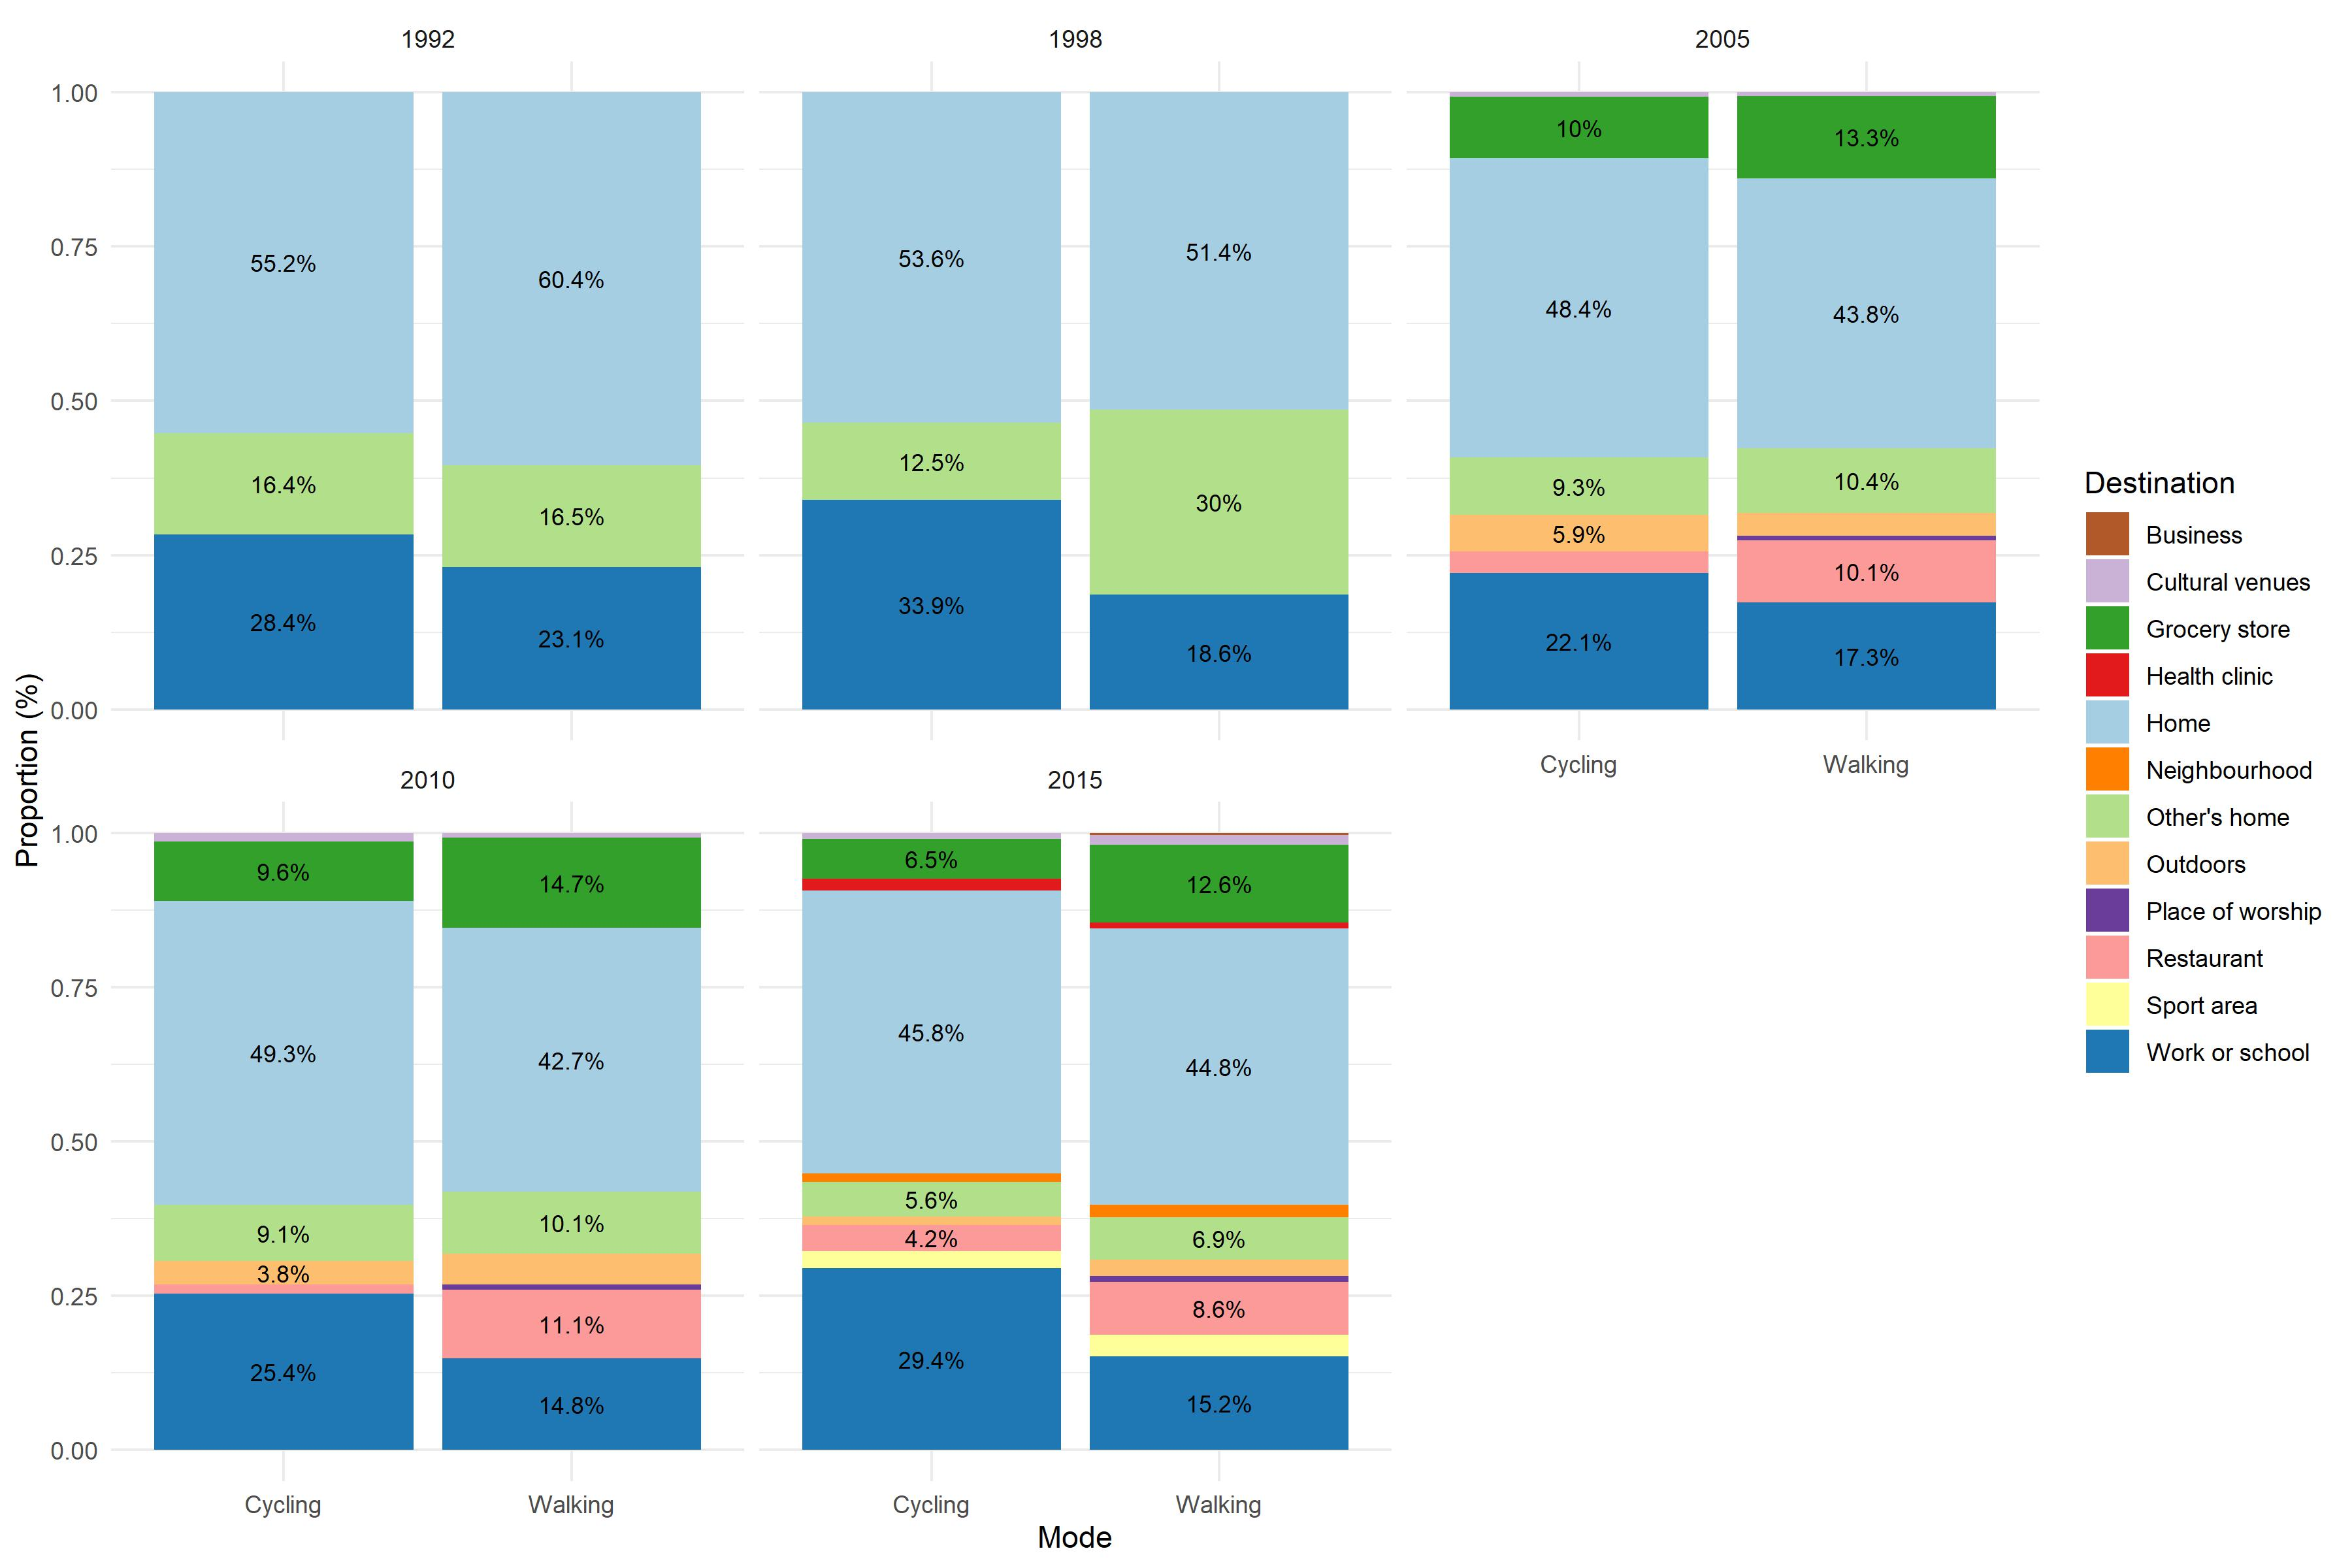
\includegraphics[width=1\linewidth]{figures/destination_percentual} \caption{Percentage of walking and cycling trips categorized by destination and year}\label{fig:figure-destmodeyearperc}
\end{figure}

After 2005, the expansion of the destination highlights some new popular
locations. For example, `Grocery store' appears as the third most chosen
destination, varying from almost 10\% in 2005 to 5.6\% in 2015 for
cycling trips and from 12\% to 10.6\% for walking trips. When
considering walking trips, `Restaurants' appears as another well chosen
destination and, in the case of cycling trips, `Outdoors' appears as a
well chosen destination.

Figure \ref{fig:figure-boxplot} present the box plot graphs showing the
travel time distribution for active transportation modes over the years,
categorized by destination. Over the period studied, the typical
duration of walking trips was consistently lower than that of cycling
trips. Some destinations are presented in only one survey, such as
`Business', `Health clinic', `Neighbourhood,' and `Sport area'. These
new destination exhibit typical walking travel times 10 minutes. For
cycling trips, `Business' recorded no trips, and while `Neighbourhood'
registered a typical travel times of 30 minutes, the others cited
destinations obtained a typical travel time of 15 minutes.

\begin{figure}

\includegraphics[width=1\linewidth]{figures/destination_boxplots} \caption{Percentage of walking trips categorized by origin and destination}\label{fig:figure-boxplot}
\end{figure}

For destinations included in more than one survey, we can compare the
temporal evolution of travel times. Starting with walking trips, we note
a trend of increasing travel times for `Restaurants' and `Outdoors'
(both increasing from 5 minutes in 2005 to 10 minutes in 2015), `Other's
home' (rising to 10 minutes in 2015 after being 5 minutes since 1992),
`Cultural venues' (from 10 minutes in 2005 and 2010 to 15 minutes in
2015), and `Place of worship' (increasing from 10 minutes in 2005 to 20
minutes in 2015). Other destinations remained constant over time for
this active travel mode, such as `Home', which, after a decline compared
to 1992, remained constant at 10 minutes from 2005 onward as the typical
travel time. `Work or school' and `Grocery store' also remained constant
at 10 minutes each since their first appearance in the GSS surveys. In
general, while `Place of worship' displayed the highest median travel
time of 20 minutes, the general median walking time cutoff appears to be
10 minutes, with most trips occurring below this limit. In this case, no
destination shows a decrease in typical travel (median) time.

For cycling trips, only `Cultural venues' did not show an increase in
typical travel time when comparing 2015 to 2010. In this case, the
travel time dropped from 25 minutes in 2010 to 15 minutes in 2015,
although it is still higher than the value measured in 2005 (10
minutes). An increasing trend in travel times is evident for
destinations such as `Grocery store' (rising from 10 to 15 minutes
between 2005 and 2015) and `Restaurant' (15 minutes in 2005 and 2010,
rising to 20 minutes in 2015). Other destinations seem to follow a
similar pattern, where higher travel times were recorded in the earlier
survey cycles, dropping over time, and then rising again in the most
recent surveys, especially in 2015. This is the case for `Home,' which
returned to the 1992 typical travel time of 20 minutes after dropping to
10 minutes in 2010. It is also worth mentioning `Work or school,' which
had a typical cycling travel time of 15 minutes in 1992, peaked at 30
minutes in 1998, dropped back to 15 minutes in 2005 and 2010, and then
increased to 20 minutes in 2015. In this case, no destination shows a
decrease in typical (median) travel time. `Outdoors' presented the
longest typical travel time for cycling, reaching a median of 30 minutes
in 2015.

Figures \ref{fig:walking-heatmap} and \ref{fig:cycling-heatmap} show
walking and cycling trips from 1992 to 2015 through heat maps. These
maps use color gradients to represent the percentage of trips between
origins and destinations, with darker colors indicating higher
percentages and lighter colors representing less frequent routes. In
1992, walking trips with `Home' as both the origin and destination made
up the majority, accounting for almost 31\% of all walking trips. These
trips often involved leisure activities, like short walks or dog
walking. Following this, trips from `Home' to `Work or school' comprised
18\% of walking trips. Overall, `Home' is the principal hub, either as
an origin or destination, with only 7\% of trips not involving `Home.'
By 1998, more than half of walking trips were between `Home' and
`Other's home,' with `Home' to `Other's home' and `Other's home' to
`Home' each representing 26\% of trips. During this year, `Home' to
`Home' accounted for only 10\% of trips. In 2005, trips with origins or
destinations involving `Home' and `Work or school' remained as the most
common, but the introduction of new destinations led to a more dispersed
trip distribution. Together, these two combinations accounted for 25\%
of all trips. In 2010, trips between `Home' and `Work or school'
continued as the most common type, representing 18\% of trips, tied with
trips from `Grocery store' to `Home' (9\%). Finishing the walking trip
descriptive analysis, in 2015, the highest proportion of trips were from
`Home' to `Work or school' (12\%) and vice versa (11\%). Trips from
`Home' to `Home' accounted for 8\% of trips, and `Grocery store' became
a notable destination for trips originating from `Home' (8\%).

\begin{figure}
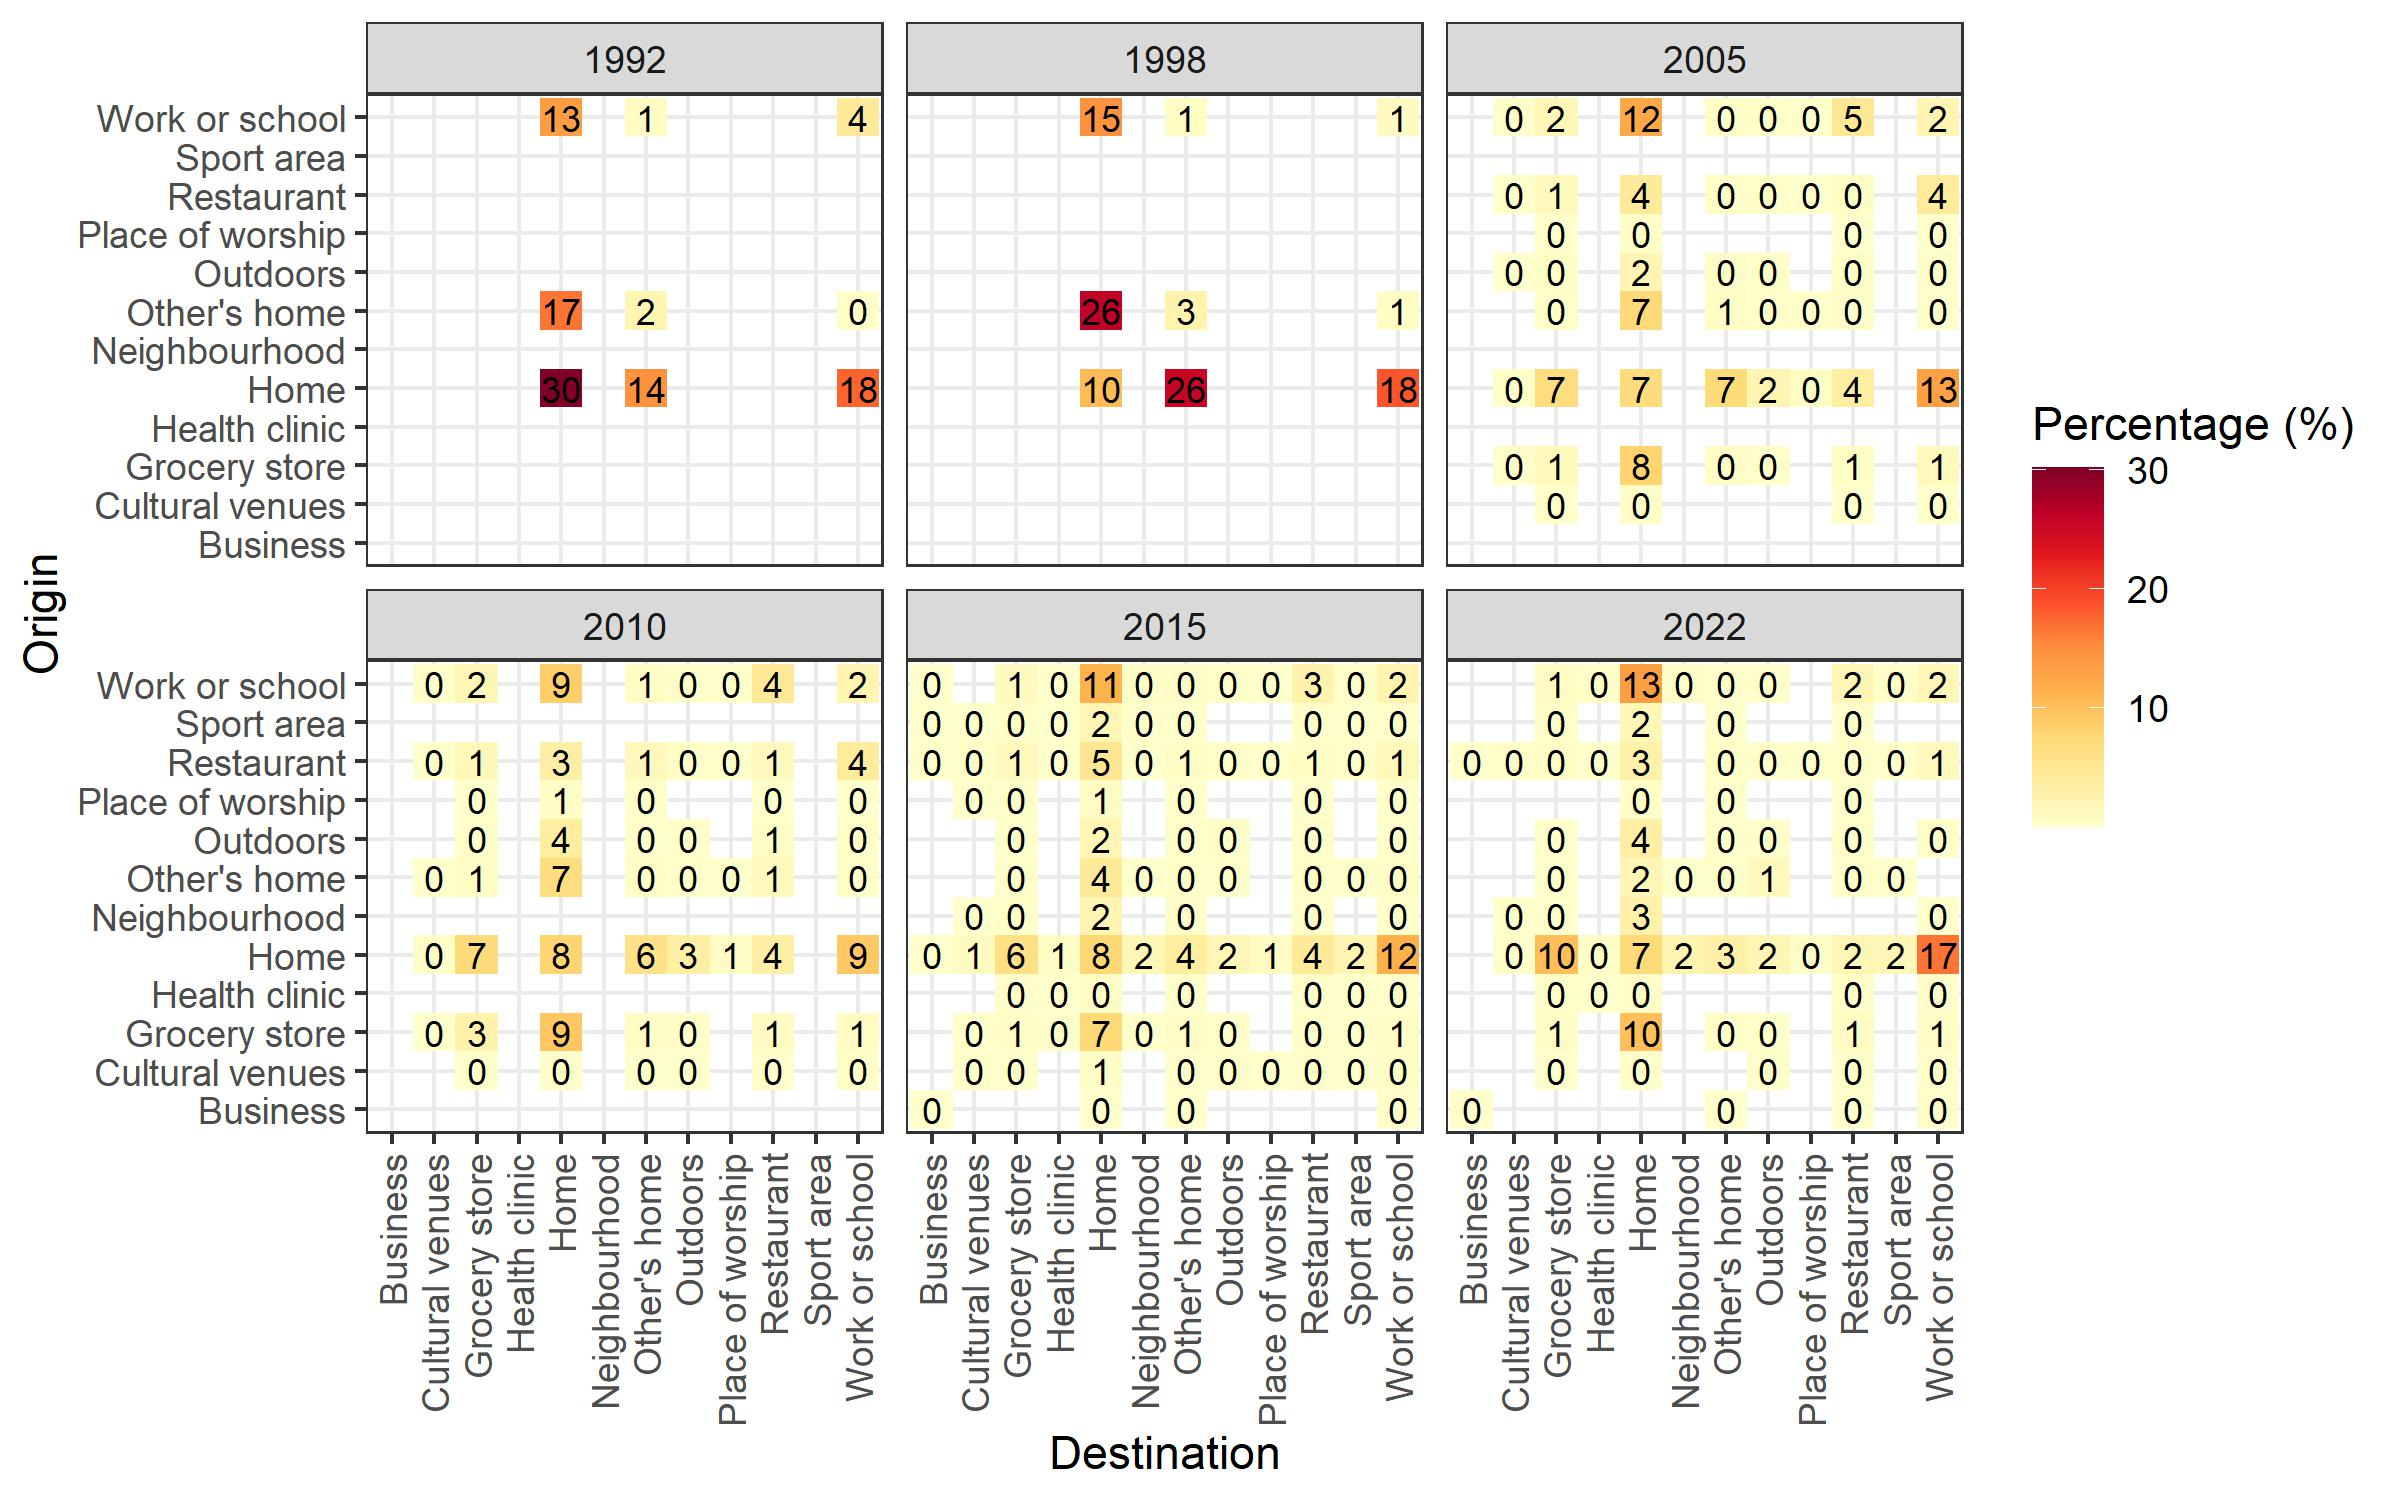
\includegraphics[width=1\linewidth]{figures/walking_hm_fig} \caption{Percentage of walking trips categorized by origin and destination}\label{fig:walking-heatmap}
\end{figure}

\begin{figure}
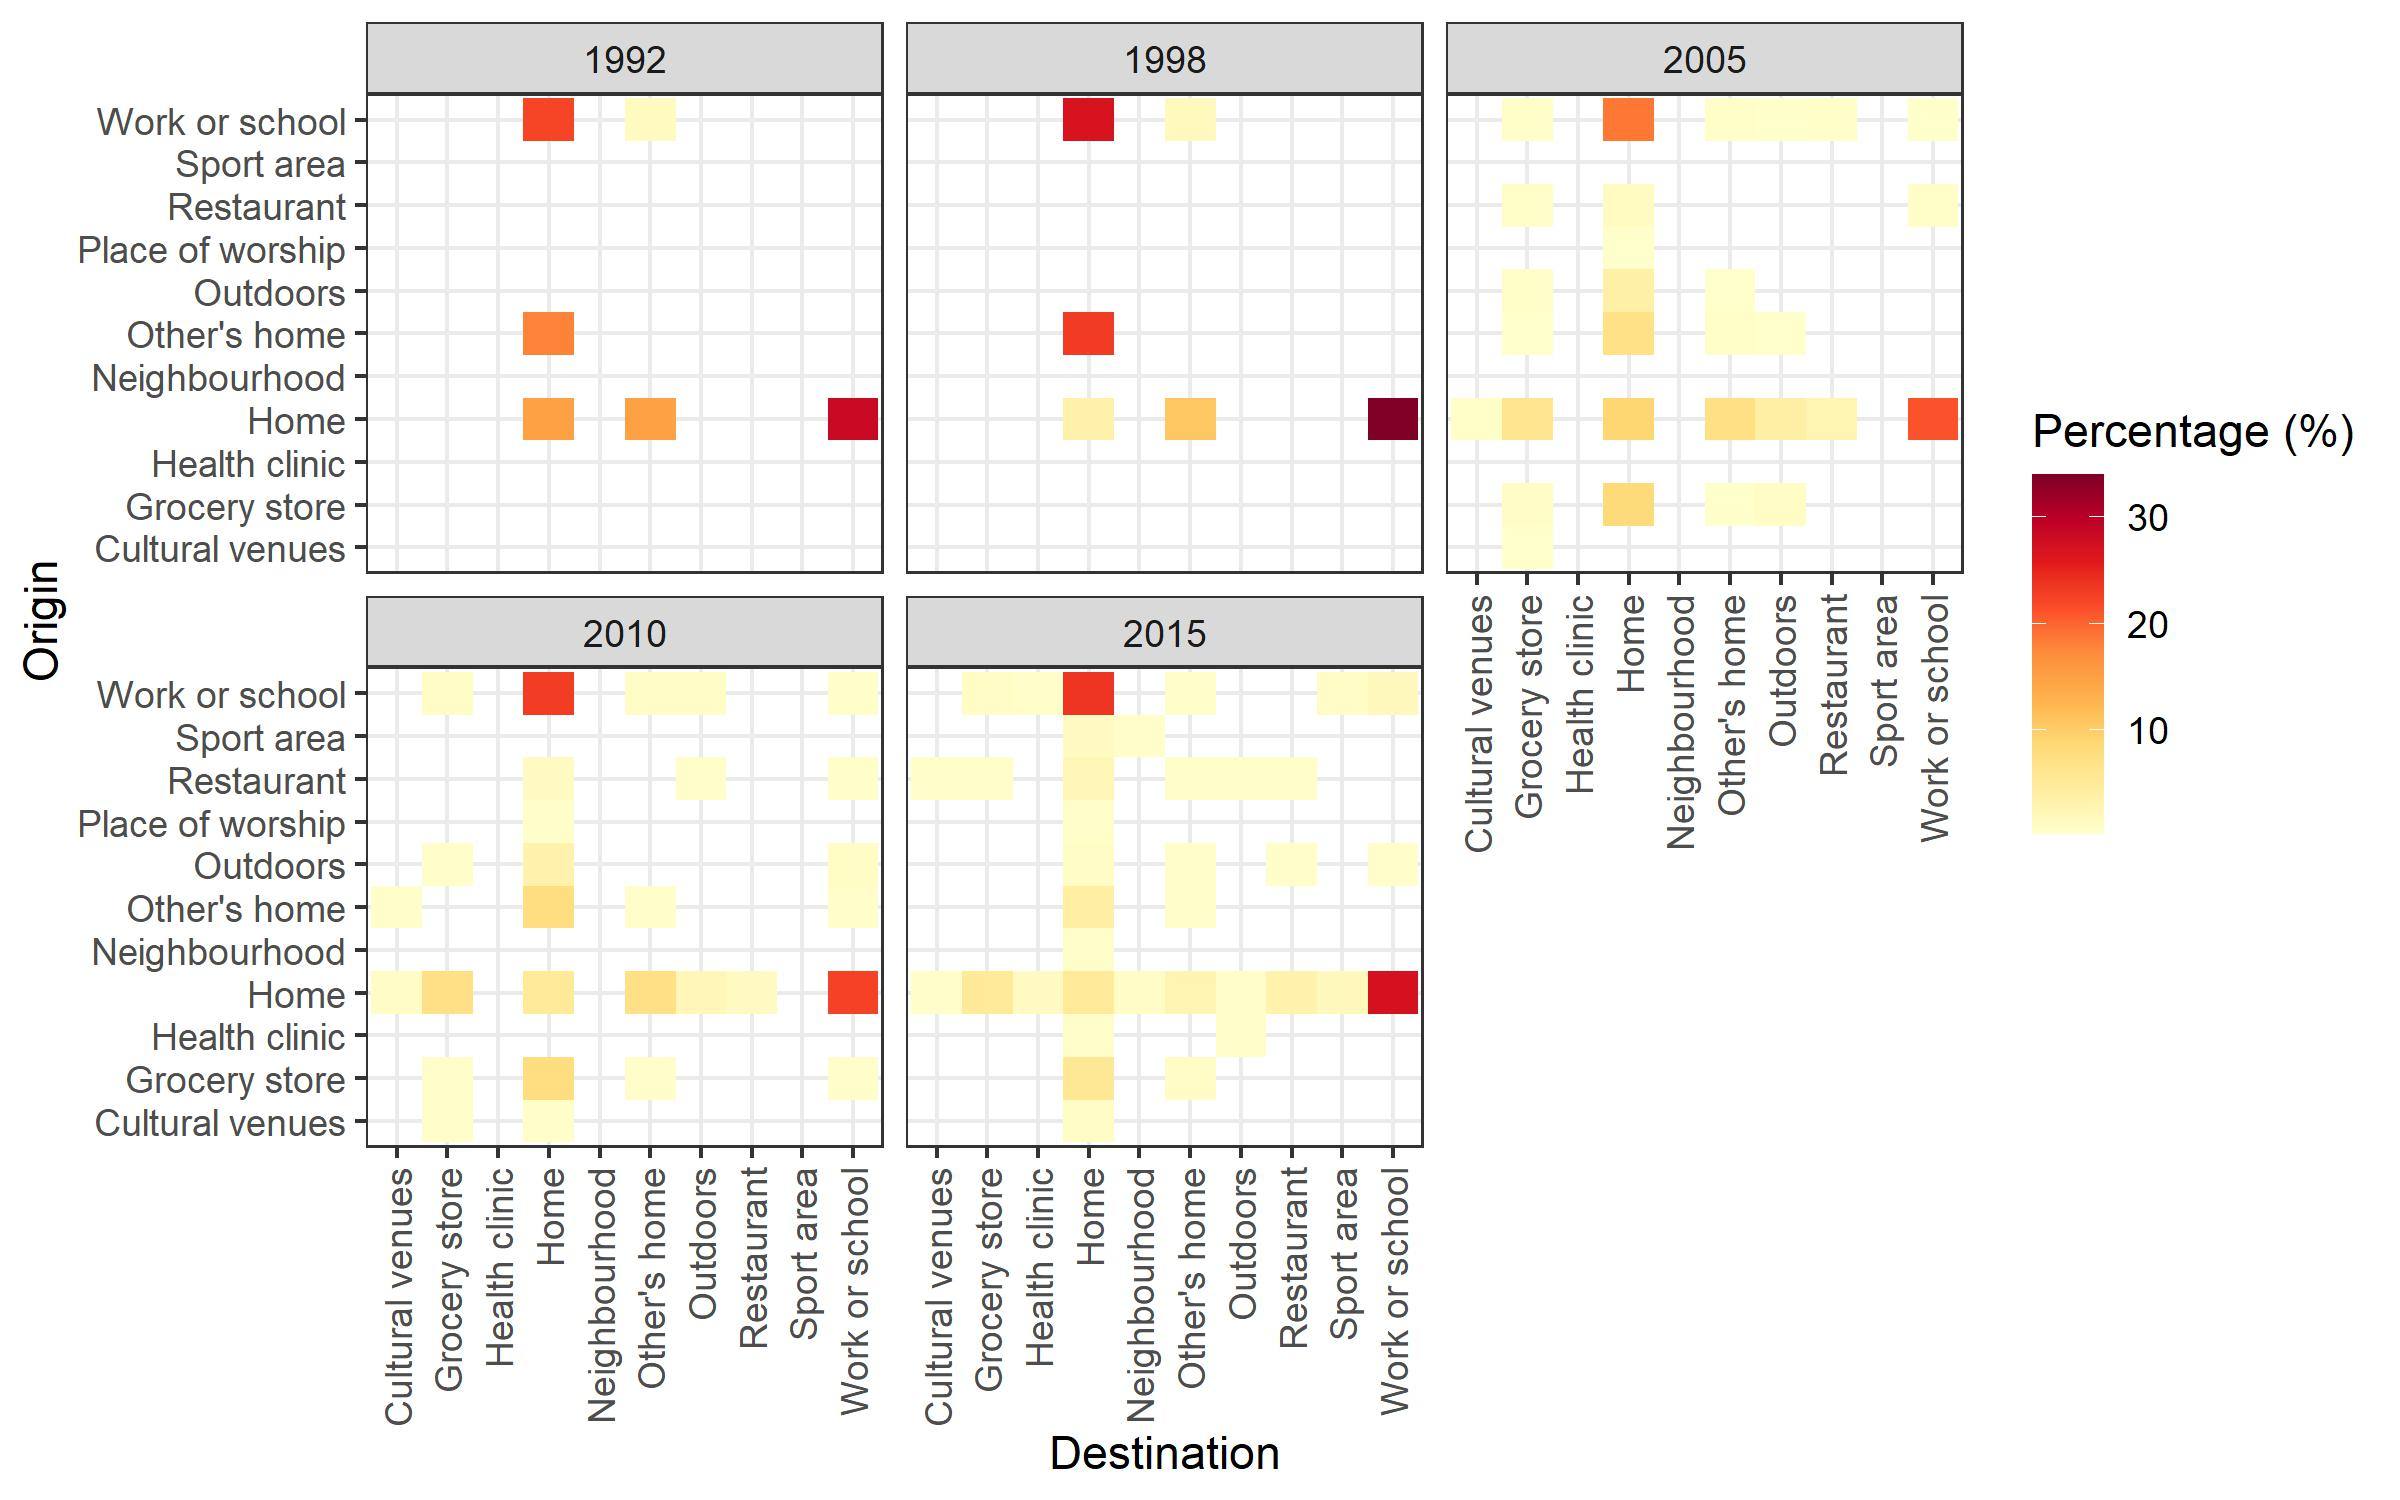
\includegraphics[width=1\linewidth]{figures/cycling_hm_fig} \caption{Percentage of walking trips categorized by origin and destination}\label{fig:cycling-heatmap}
\end{figure}

For cycling trips (Figure \ref{fig:cycling-heatmap}), in 1992, the most
common trip was from `Home' to `Work or school' (26\%), followed by
trips from `Other's home' to `Home' (22\%). In all following years, the
most frequent trip were between `Home' and `Work or school' in both
direction. This combination accounted for 65\% of the trips in 1998,
40\% in 2005, 52\% in 2010, and 58\% in 2015. Additionally and unlike
walking trips, `Home' to `Home' trips were not a common cycling trip in
any of the surveys. This suggests that leisure trips, such as activities
around the home, are predominantly done by foot rather than by bicycle.

We analyzed whether the temporal differences in travel times for the
destinations had statistical significance. Only destinations that appear
in more than one year can have their temporal evolution analyzed.
Therefore, from the twelve possible destinations, in the cycling mode
only seven locations can be temporally analyzed: `Cultural venues,'
`Grocery store,' `Home,' `Other's home,' `Outdoors,' `Restaurant,' and
`Work or school.' In the case of walking trips, it is possible to
include `Place of worship' to the previous destination list.

After performing the Kruskal-Wallis test (to assess whether there was a
statistically significant difference between the distributions of
empirical travel time values, considering the time differences for each
destination and the weight of each episode) and the pairwise Wilcoxon
test, we were able to identify the destinations where a statistically
significant difference was detected. Table \ref{tab:result-stats} shows
only the destinations where a statistically significant difference was
found, considering the two modes of active transport analyzed.

For both active transportation modes, the possible destinations had at
least two year with statistically significant difference in travel
times. Considering the cycling mode and, for instance, the ``Home''
destination, there was a statistically significant difference (p-value
\textless{} 2.2e-16) for every possible combination of two survey
cycles. This result indicates that the previously discussed increase in
typical cycling travel time for home destinations when compared 2015 to
2010 is statistically significant. As identified for cycling trips, all
destinations presented at least two years with statistically significant
difference in travel times for walking trips (p-value \textless{}
2.2e-16).

\begin{table}
\centering
\caption{\label{tab:kruskal-walking}\label{tab:result-stats}P-values of the pairwise Wilcoxon test .}
\centering
\resizebox{\ifdim\width>\linewidth\linewidth\else\width\fi}{!}{
\fontsize{10}{12}\selectfont
\begin{tabular}[t]{lllrrrr}
\toprule
Mode & Destination & Year & 1992 & 1998 & 2005 & 2010\\
\midrule
 & Restaurant & 2010 &  &  & 0 & \\

 & Restaurant & 2015 &  &  & 0 & 0\\

 & Grocery store & 2010 &  &  & 0 & \\

 & Grocery store & 2015 &  &  & 0 & 0\\

 & Home & 1998 & 0 &  &  & \\

 & Home & 2005 & 0 & 0 &  & \\

 & Home & 2010 & 0 & 0 & 0 & \\

 & Home & 2015 & 0 & 0 & 0 & 0\\

 & Work or school & 1998 & 0 &  &  & \\

 & Work or school & 2005 & 0 & 0 &  & \\

 & Work or school & 2010 & 0 & 0 & 0 & \\

 & Work or school & 2015 & 0 & 0 & 0 & 0\\

 & Cultural venues & 2010 &  &  & 0 & \\

 & Cultural venues & 2015 &  &  & 0 & 0\\

 & Other's home & 1998 & 0 &  &  & \\

 & Other's home & 2005 & 0 & 0 &  & \\

 & Other's home & 2010 & 0 & 0 & 0 & \\

 & Other's home & 2015 & 0 & 0 & 0 & 0\\

 & Place of worship & 2010 &  &  & 0 & \\

 & Place of worship & 2015 &  &  & 0 & 0\\

 & Outdoors & 2010 &  &  & 0 & \\

\multirow[t]{-22}{*}{\raggedright\arraybackslash Walking} & Outdoors & 2015 &  &  & 0 & 0\\
\cmidrule{1-7}
 & Restaurant & 2010 &  &  & 0 & \\

 & Restaurant & 2015 &  &  & 0 & 0\\

 & Home & 1998 & 0 &  &  & \\

 & Home & 2005 & 0 & 0 &  & \\

 & Home & 2010 & 0 & 0 & 0 & \\

 & Home & 2015 & 0 & 0 & 0 & 0\\

 & Work or school & 1998 & 0 &  &  & \\

 & Work or school & 2005 & 0 & 0 &  & \\

 & Work or school & 2010 & 0 & 0 & 0 & \\

 & Work or school & 2015 & 0 & 0 & 0 & 0\\

 & Other's home & 1998 & 0 &  &  & \\

 & Other's home & 2005 & 0 & 0 &  & \\

 & Other's home & 2010 & 0 & 0 & 0 & \\

 & Other's home & 2015 & 0 & 0 & 0 & 0\\

 & Cultural venues & 2010 &  &  & 0 & \\

 & Cultural venues & 2015 &  &  & 0 & \\

 & Outdoors & 2010 &  &  & 0 & \\

 & Outdoors & 2015 &  &  & 0 & 0\\

 & Grocery store & 2010 &  &  & 0 & \\

\multirow[t]{-20}{*}{\raggedright\arraybackslash Cycling} & Grocery store & 2015 &  &  & 0 & 0\\
\bottomrule
\end{tabular}}
\end{table}

\subsubsection{Population with records of active
trip}\label{population-with-records-of-active-trip}

In general, the share of the population with active trip records varied
between 7.8\% and 14.5\% from 1992 to 2015 (Table
\ref{tab:active-pop-proportion-table}). The year 1998 recorded the
lowest level of active trip participation, with 7.8\% (1,892,299
people), while 2010 marked the peak of active participation at 14.5\%
(4,084,114 people). In 2015, the trend of increasing participation in
walking or cycling trips, which began after the 1998 low and peaked in
2010, appeared to pause. In that year, the most recent in the analysis,
around 11\% of the population (3,265,846 people) recorded at least one
active trip.

The number of people with active trip episodes is mainly influenced by
walking episodes. Over 90\% of the recorded active trips involve
individuals with walking episodes. However, the percentage patterns for
the population with records of walking and cycling trips do not differ
significantly from those observed when both modes are considered
together.

\begingroup\fontsize{6}{8}\selectfont

\begin{longtable}[t]{rrrrrrrrrrrrrr}
\caption{\label{tab:active_pop_proportion_table}\label{tab:active-pop-proportion-table}Count and share of population with at least one active travel episode by year}\\
\toprule
\multicolumn{1}{c}{ } & \multicolumn{4}{c}{Walking} & \multicolumn{4}{c}{Cycling} & \multicolumn{4}{c}{Total} \\
\cmidrule(l{3pt}r{3pt}){2-5} \cmidrule(l{3pt}r{3pt}){6-9} \cmidrule(l{3pt}r{3pt}){10-13}
Year & Active & (\%) & Non-active & (\%) & Active & (\%) & Non-active & (\%) & Active & (\%) & Non-active & (\%) & Population\\
\midrule
1992 & 1906913 & 8.96 & 19387400 & 91.04 & 187615 & 0.88 & 21106698 & 99.12 & 2086672 & 9.80 & 19207641 & 90.20 & 21294313\\
1998 & 1751388 & 7.22 & 22508749 & 92.78 & 155191 & 0.64 & 24104946 & 99.36 & 1892299 & 7.80 & 22367838 & 92.20 & 24260137\\
2005 & 3360966 & 12.88 & 22734853 & 87.12 & 243303 & 0.93 & 25852516 & 99.07 & 3577772 & 13.71 & 22518047 & 86.29 & 26095819\\
2010 & 3877823 & 13.81 & 24197788 & 86.19 & 284567 & 1.01 & 27791044 & 98.99 & 4084114 & 14.55 & 23991496 & 85.45 & 28075610\\
2015 & 3068296 & 10.31 & 26698103 & 89.69 & 262317 & 0.88 & 29504081 & 99.12 & 3265846 & 10.97 & 26500553 & 89.03 & 29766399\\
\bottomrule
\end{longtable}
\endgroup{}

Considering only the population with records of walking episodes, Figure
\ref{fig:walking-population-by-year-destination-fig} shows that, in all
the years analyzed, ``Home'' and ``Work or study'' were the main
destinations (as previously discussed in the previous subsection). Those
who recorded only one trip accounted for approximately 84\% of the
population, around 13\% recorded more than one walking trip, and the
remaining 2 to 3\% recorded three or more trips. The maximum number of
walking trips registered by a person was 10 episodes (in 1992, 2005, and
2010). In contrast, 2015 shows a reduction compared to previous years,
with a maximum of 8 walking trips recorded by a single person. In all
these maximum cases, the destination was ``Home.''

\begin{figure}

{\centering 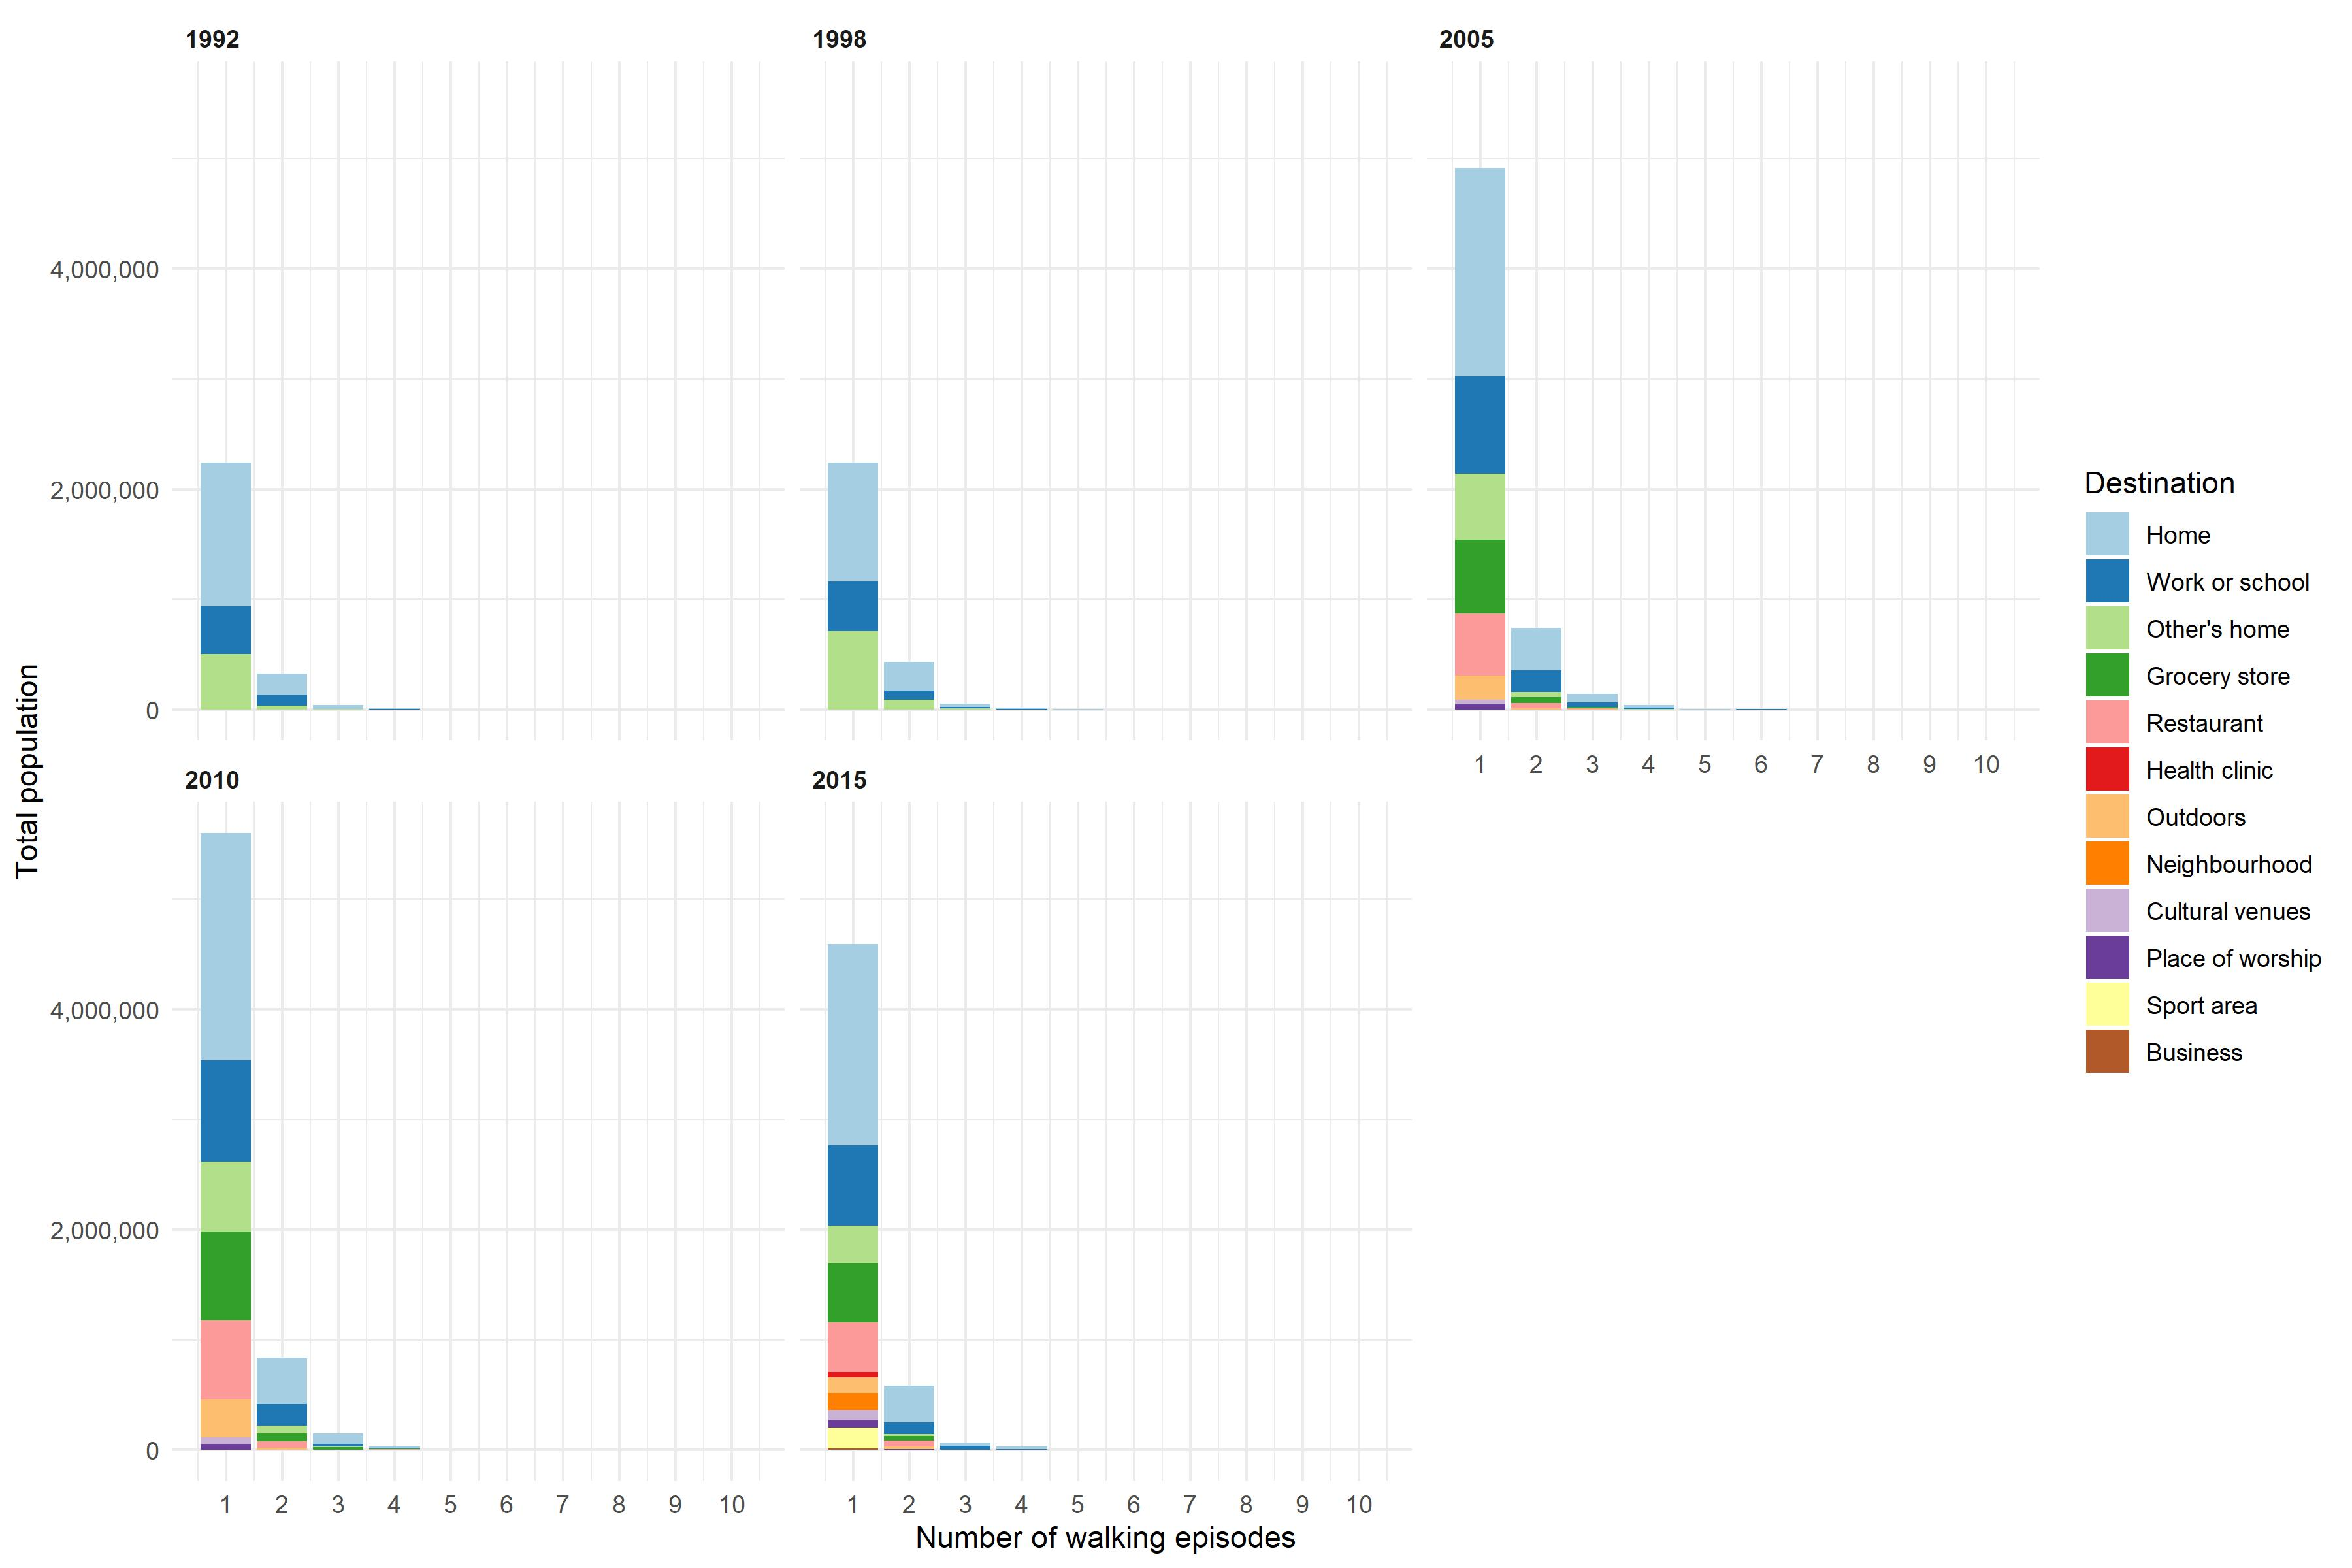
\includegraphics[width=1\linewidth]{figures/people_per_ep_walking} 

}

\caption{Number of people with at least one walking episodes, by destination and year.}\label{fig:walking-population-by-year-destination-fig}
\end{figure}

For the cycling population, the maximum number of trips recorded was 4,
in 2005 (to ``Home'' and ``Grocery store,'' as shown in Figure
\ref{fig:cycling-population-by-year-destination-fig}). This maximum
value is lower compared to the walking population, and there is a higher
concentration of cyclists recording only one episode (around 90\%), two
episodes (around 8\%), and the remaining 2--3\% recording three or four
trips.

\begin{figure}

{\centering 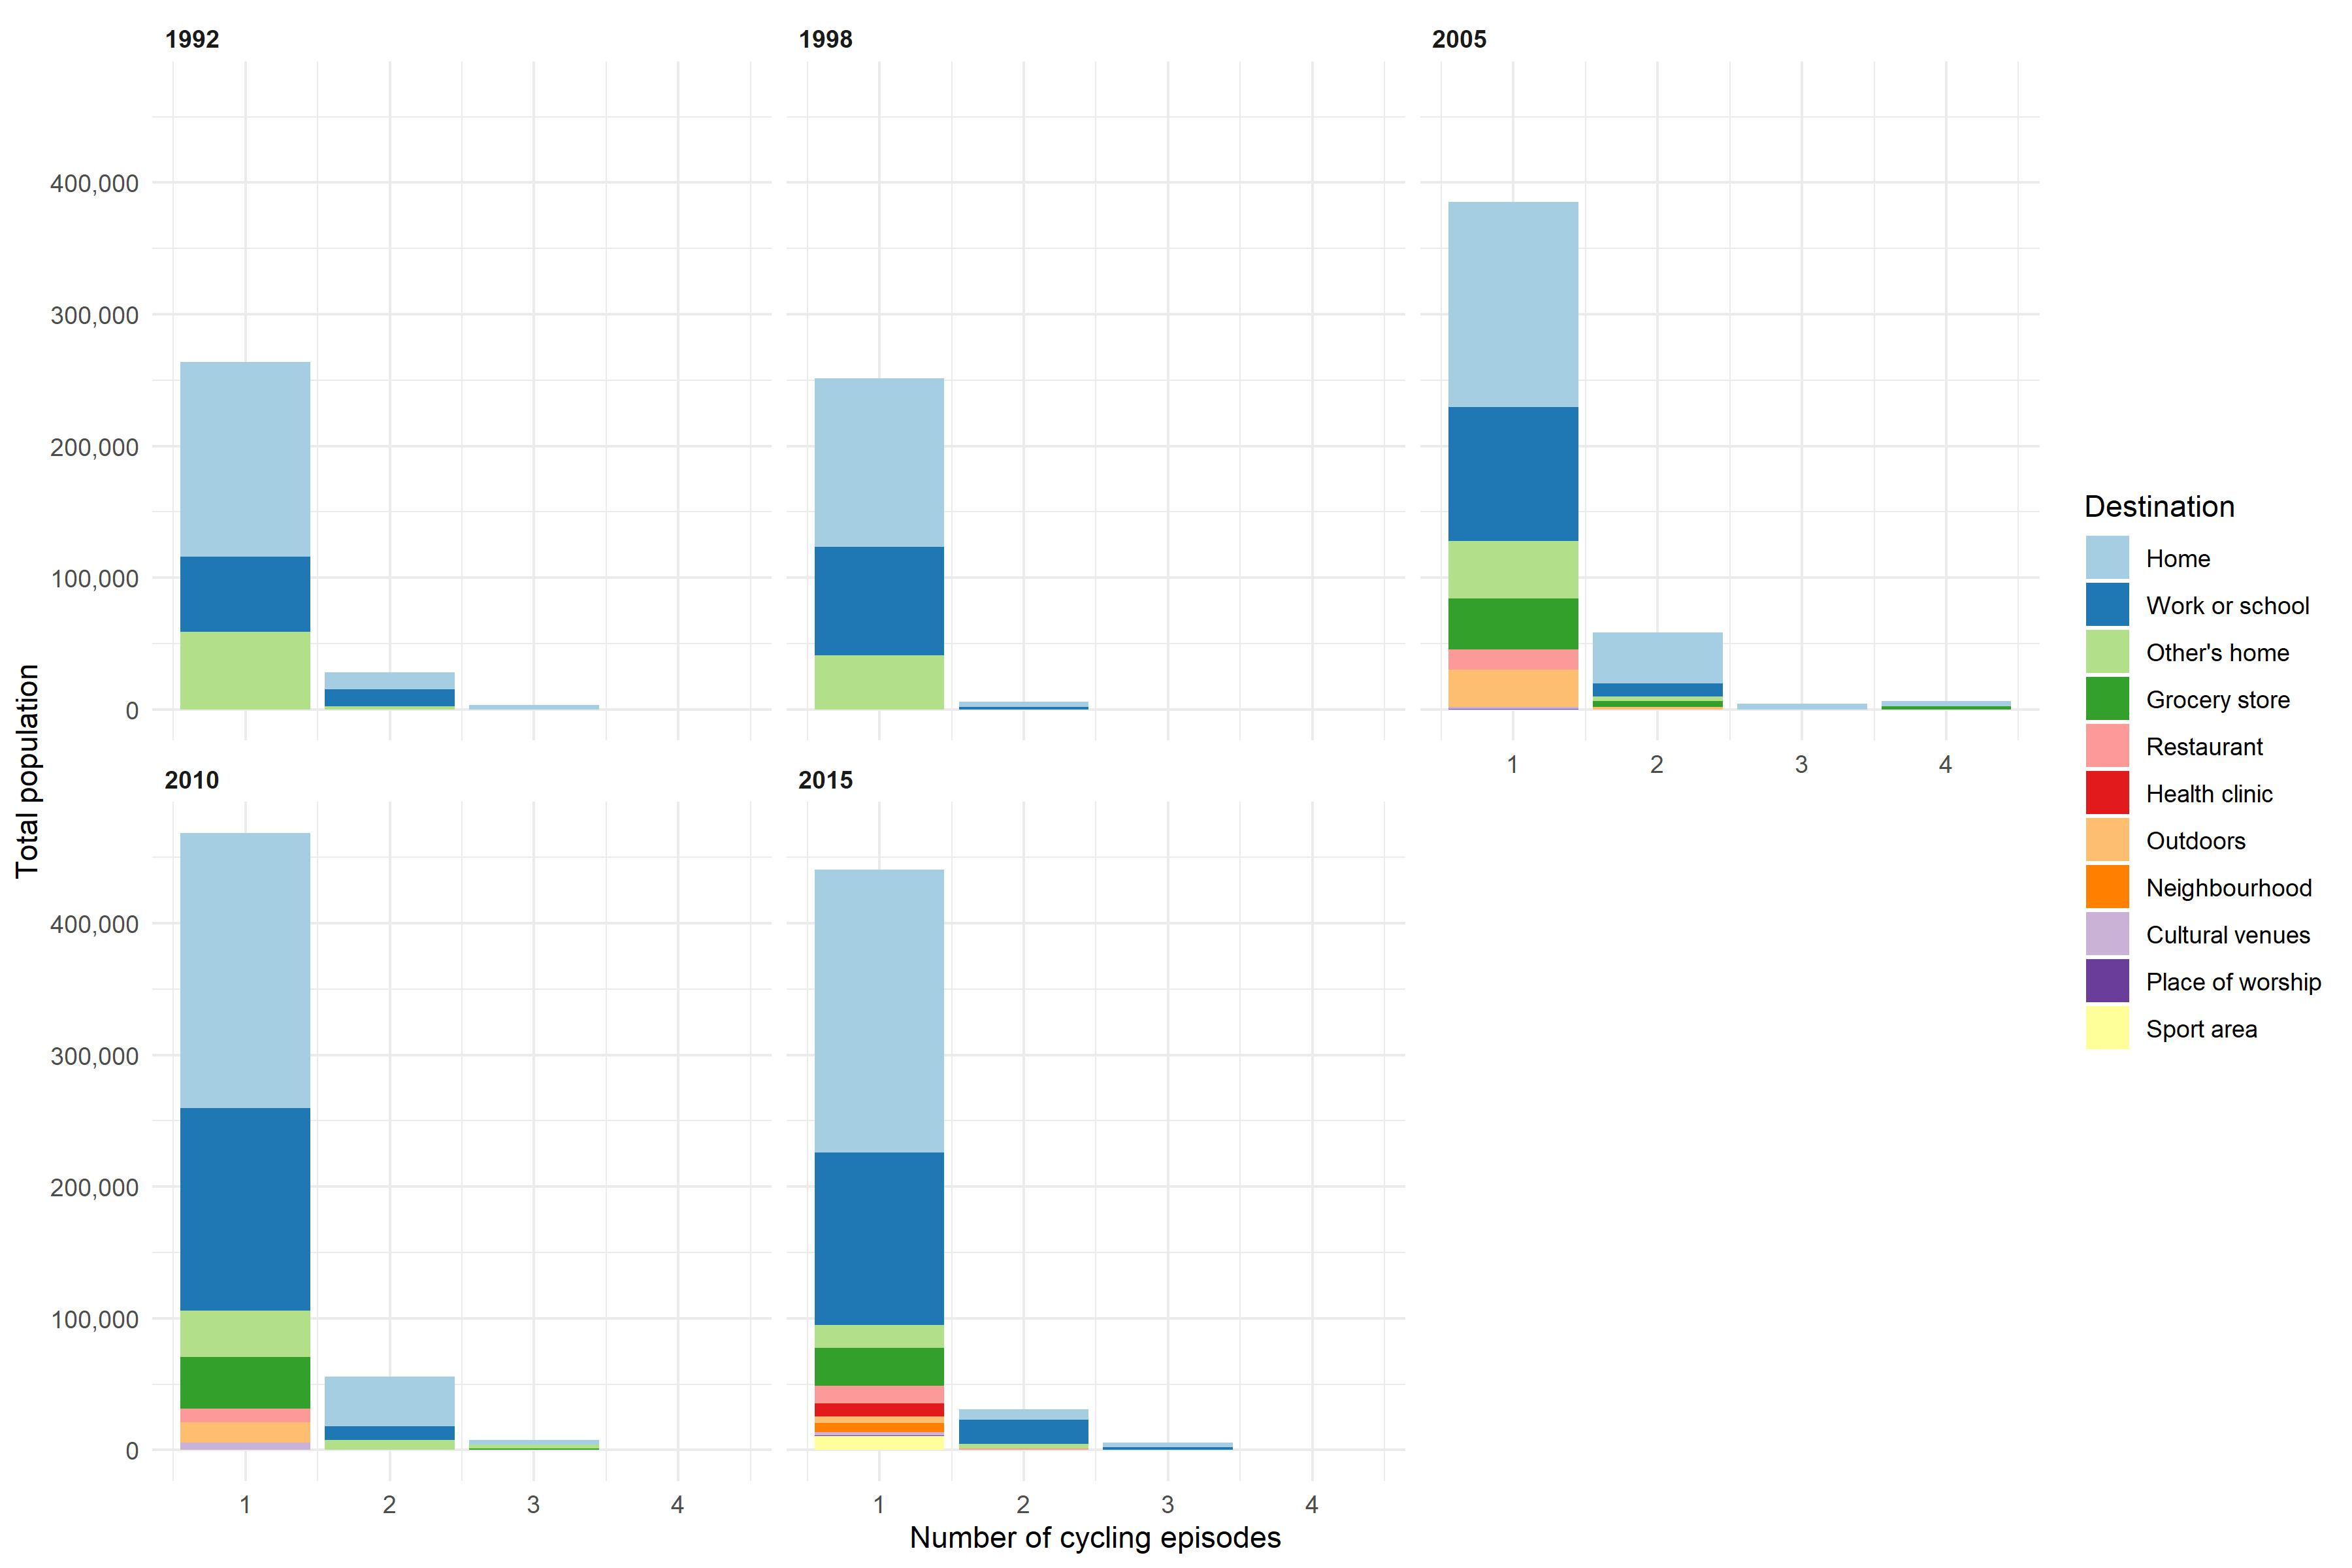
\includegraphics[width=1\linewidth]{figures/people_per_ep_cycling} 

}

\caption{Number of people with at least one cycling episodes, by destination and year.}\label{fig:cycling-population-by-year-destination-fig}
\end{figure}

Analyzing the number of episodes per person for the general population,
the value is close to 0, ranging from a minimum of 0.009 in 2015 to a
maximum of 0.026 in 1992. Considering only the population with active
episodes recorded, this value is approximately 1.180 active episodes per
person, varying from a maximum of 1.203 episodes in 2005 to a minimum of
1.152 episodes per person in 2015. Figure \ref{fig:eps-per-person-fig}
presents these values broken down by mode, walking and cycling.

Since walking episodes form the majority of active trip episodes, the
pattern for the walking population is similar to the general trend. For
the cycling population, only the low value observed in 1992 for the
active population appears different from the overall pattern. However,
the number of cyclists in 1992 was not sufficient to alter the overall
trend for the active population. These statistics reveal a trend of
decreasing active trips (whether walking or cycling) when comparing data
from 1992 to 2005, with a particularly noticeable decline after 1992 for
walking and 2005 for cycling.

\begin{figure}

{\centering 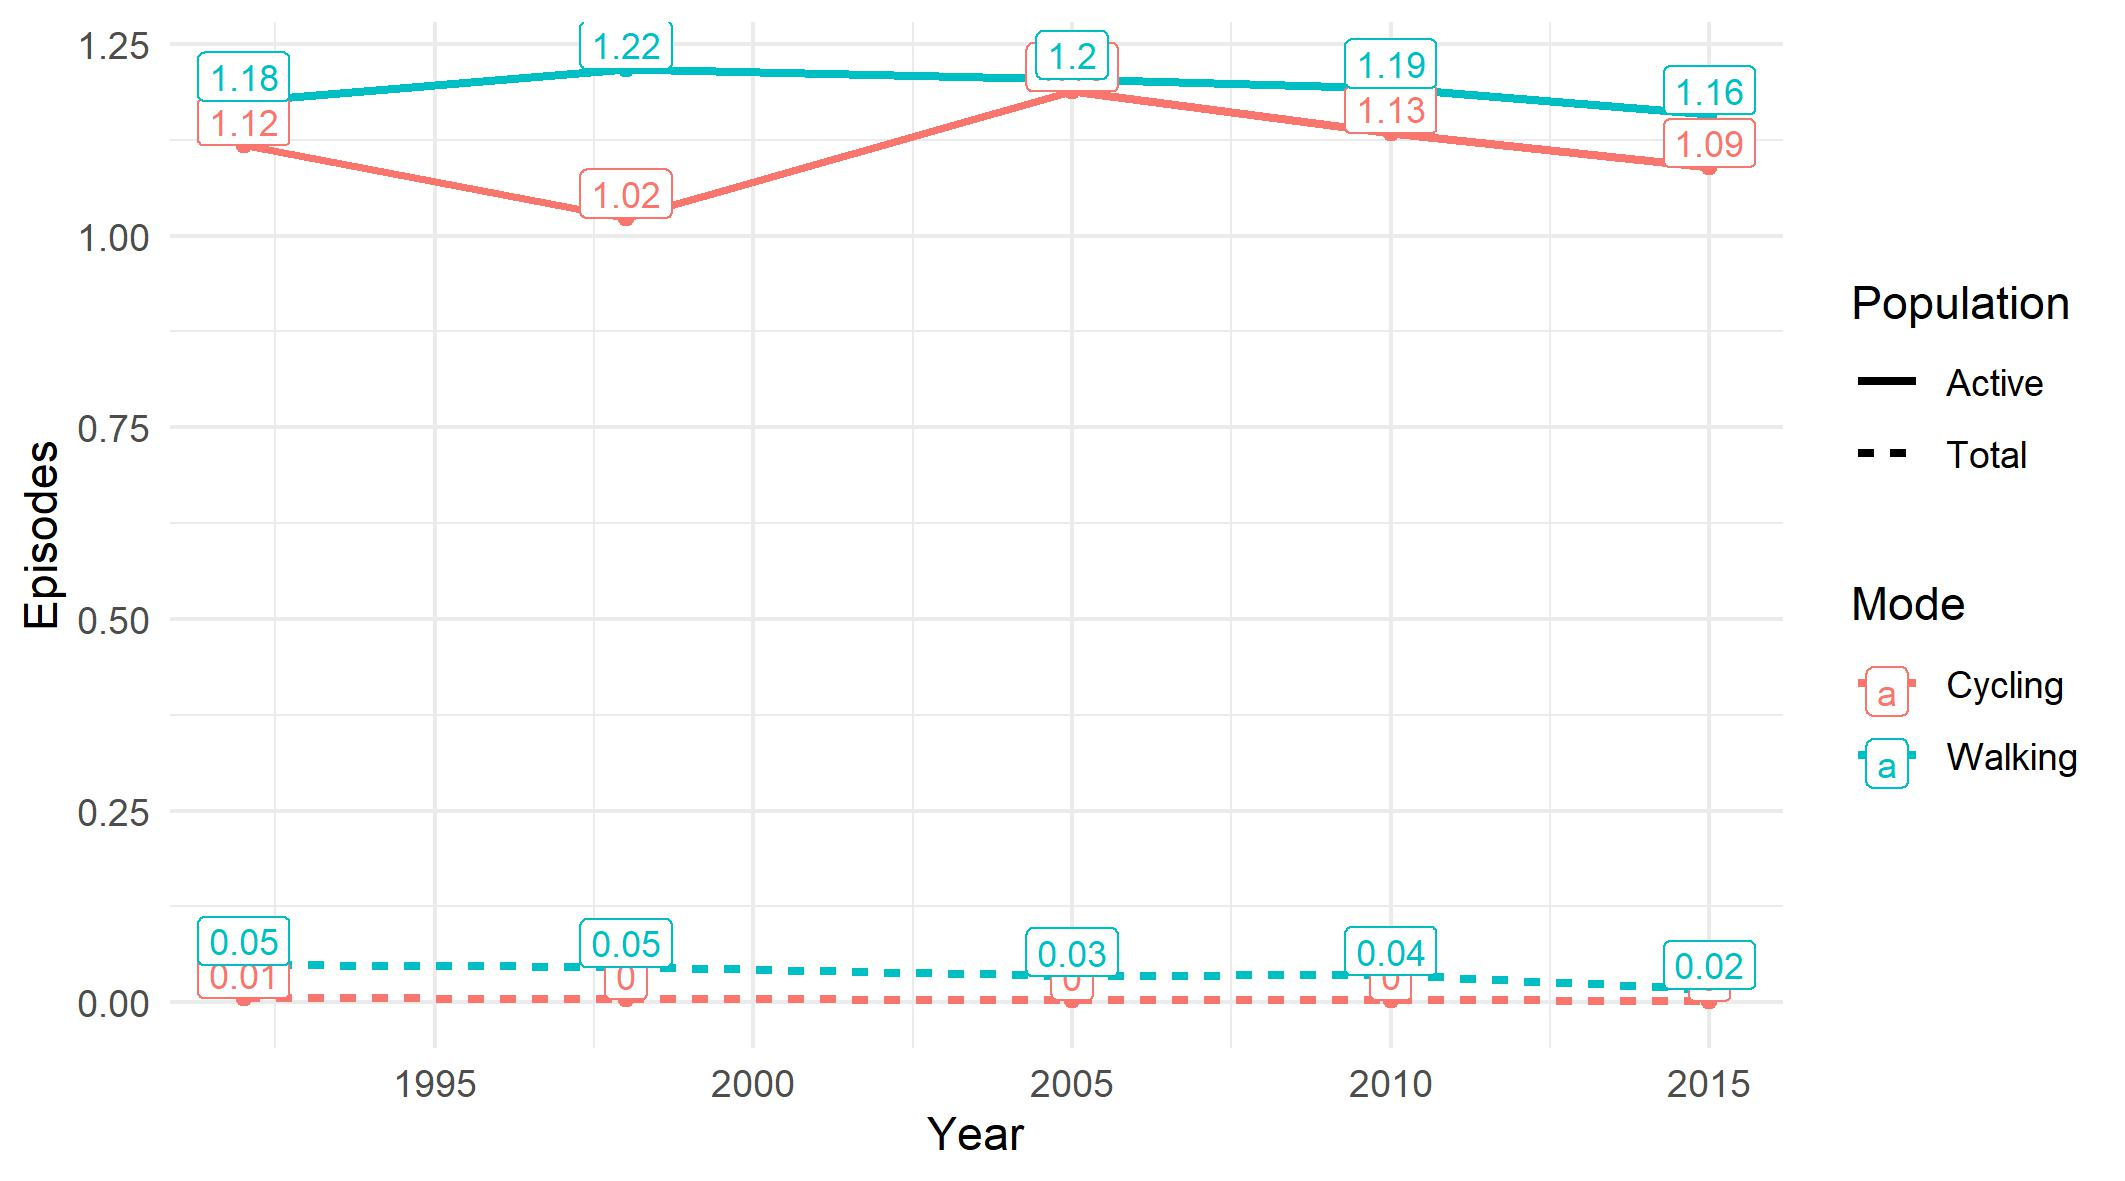
\includegraphics[width=1\linewidth]{figures/episodes_per_person} 

}

\caption{Number of active episodes by person.}\label{fig:eps-per-person-fig}
\end{figure}

\subsection{Calibrated impedance
function}\label{calibrated-impedance-function}

This section presents the identified impedance functions for walking and
cycling trips to various destinations across Canadian Metropolitan and
Census Agglomeration Areas from 1992 to 2015. In general, the impedance
functions aim to capture transportation behavior, illustrating that the
likelihood of traveling between two points decreases as travel duration
increases. Each impedance function follows one of the mathematical
equations previously mentioned, enabling the plotting of PDF curves.
These curves also highlight critical points at which a person's tendency
to walk or cycle significantly decreases.

As explained in the methodology section, we used the
\texttt{fitdistrplus} package (Delignette-Muller and Dutang 2015) to
calibrate the functions. We selected the best impedance function for
each transportation mode, destination, and year based on the lowest
Akaike Information Criterion (AIC) value (Akaike 1974). The AIC metric
not only assesses the goodness of fit but also penalizes model
complexity to prevent overfitting. AIC provides a balance between a
model's accuracy and simplicity, with lower values indicating a more
economical model. The distribution with the lowest AIC was considered
the most suitable for representing the distance decay curve for each
specific destination in each year. We chose AIC as the selection
criterion because, while the \texttt{fitdistrplus} package accommodates
weighted episodes during estimation, it does not extend this
functionality to diagnostic plots, which are typically unweighted and
traditionally used to select the best-fitting function.

In total, we fitted 64 impedance functions. Among the candidate
distributions, only the lognormal, gamma, and uniform distributions were
selected, with the uniform distribution being chosen exclusively for
certain cycling destinations. The absence of exponential functions,
given the variety of destinations, year and mode of transport, indicates
that the impedance functions applied in active accessibility studies may
not be adequately measuring travel behavior, especially for cases when
the travel time is close to 0 minute. Table
\ref{tab:walking-functions-tab} displays the selected functions for
walking trips, while Table \ref{tab:cycling-functions-tab} presents the
functions for cycling trips. Appendix A includes the AIC, BIC, and
log-likelihood values for all candidate distributions.

\begin{table}
\centering
\caption{\label{tab:selected_functions}\label{tab:walking-functions-tab}Impedance functions and AIC for walking trips.}
\centering
\resizebox{\ifdim\width>\linewidth\linewidth\else\width\fi}{!}{
\fontsize{10}{12}\selectfont
\begin{threeparttable}
\begin{tabular}[t]{rllrrrr}
\toprule
\multicolumn{1}{c}{\textbf{Year}} & \multicolumn{1}{c}{\textbf{Destination}} & \multicolumn{1}{c}{\textbf{Impedance function}} & \multicolumn{1}{c}{\textbf{Parameter 1*}} & \multicolumn{1}{c}{\textbf{Parameter 2*}} & \multicolumn{1}{c}{\textbf{AIC}} & \multicolumn{1}{c}{\textbf{Count}}\\
\midrule
 & Home & Lognormal & 2.92 & 0.77 & 7761103 & 296\\

 & Other's home & Lognormal & 2.15 & 0.84 & 1778150 & 81\\

\multirow[t]{-3}{*}{\raggedleft\arraybackslash 1992} & Work or school & Lognormal & 2.38 & 0.70 & 2319400 & 113\\
\cmidrule{1-7}
 & Home & Lognormal & 2.07 & 0.92 & 5656275 & 302\\

 & Other's home & Lognormal & 1.75 & 0.97 & 2892771 & 176\\

\multirow[t]{-3}{*}{\raggedleft\arraybackslash 1998} & Work or school & Gamma & 1.23 & 0.09 & 2318752 & 109\\
\cmidrule{1-7}
 & Cultural venues & Gamma & 4.10 & 0.34 & 238506 & 25\\

 & Grocery store & Gamma & 1.22 & 0.10 & 4776215 & 558\\

 & Home & Gamma & 1.16 & 0.08 & 17291041 & 1831\\

 & Other's home & Gamma & 1.03 & 0.11 & 3420742 & 436\\

 & Outdoors & Gamma & 1.24 & 0.13 & 1272012 & 155\\

 & Place of worship & Gamma & 2.07 & 0.19 & 228307 & 32\\

 & Restaurant & Lognormal & 1.95 & 0.79 & 3727576 & 421\\

\multirow[t]{-8}{*}{\raggedleft\arraybackslash 2005} & Work or school & Lognormal & 2.13 & 0.79 & 8182691 & 724\\
\cmidrule{1-7}
 & Cultural venues & Gamma & 3.60 & 0.34 & 304141 & 25\\

 & Grocery store & Lognormal & 2.08 & 0.85 & 6369652 & 489\\

 & Home & Gamma & 1.10 & 0.07 & 19584386 & 1424\\

 & Other's home & Lognormal & 1.81 & 0.92 & 4035574 & 336\\

 & Outdoors & Gamma & 1.27 & 0.13 & 2114346 & 167\\

 & Place of worship & Lognormal & 1.95 & 0.70 & 285177 & 28\\

 & Restaurant & Lognormal & 2.01 & 0.90 & 5187191 & 371\\

\multirow[t]{-8}{*}{\raggedleft\arraybackslash 2010} & Work or school & Lognormal & 2.21 & 0.78 & 7917431 & 494\\
\cmidrule{1-7}
 & Business & Lognormal & 2.41 & 0.67 & 102286 & 8\\

 & Cultural venues & Gamma & 4.57 & 0.34 & 543242 & 43\\

 & Grocery store & Lognormal & 2.48 & 0.68 & 4001111 & 338\\

 & Health clinic & Lognormal & 2.44 & 0.70 & 324578 & 27\\

 & Home & Lognormal & 2.57 & 0.74 & 17235960 & 1202\\

 & Neighbourhood & Lognormal & 2.41 & 0.77 & 981626 & 53\\

 & Other's home & Lognormal & 2.43 & 0.80 & 2388598 & 186\\

 & Outdoors & Lognormal & 2.54 & 0.79 & 1247963 & 72\\

 & Place of worship & Gamma & 5.64 & 0.28 & 343187 & 24\\

 & Restaurant & Lognormal & 2.38 & 0.74 & 3490082 & 231\\

 & Sport area & Lognormal & 2.48 & 0.59 & 1199687 & 94\\

\multirow[t]{-12}{*}{\raggedleft\arraybackslash 2015} & Work or school & Lognormal & 2.55 & 0.64 & 6612061 & 407\\
\bottomrule
\end{tabular}
\begin{tablenotes}
\item \textit{Note: } 
\item For 'lnorm' distributions, 'Parameter 1' and 'Parameter 2' refer to the mean and standard deviation of the distribution on the logarithmic scaler, respectively. For the 'Gamma' distribution, 'Parameter 1' and 'Parameter 2' refer to the rate and shape of the distribution, respectively. For the 'Uniform' distribution,  'Parameter 1' refers to the minimum lower bound and 'Parameter 2'  refers to the upper bound (maximum) of the distribution.  'AIC' means Akaike information criterion.
\end{tablenotes}
\end{threeparttable}}
\end{table}

\begin{table}
\centering
\caption{\label{tab:selected_functions}\label{tab:cycling-functions-tab}Impedance functions and AIC for cycling trips.}
\centering
\resizebox{\ifdim\width>\linewidth\linewidth\else\width\fi}{!}{
\fontsize{10}{12}\selectfont
\begin{threeparttable}
\begin{tabular}[t]{rllrrrr}
\toprule
\multicolumn{1}{c}{\textbf{Year}} & \multicolumn{1}{c}{\textbf{Destination}} & \multicolumn{1}{c}{\textbf{Impedance function}} & \multicolumn{1}{c}{\textbf{Parameter 1*}} & \multicolumn{1}{c}{\textbf{Parameter 2*}} & \multicolumn{1}{c}{\textbf{AIC}} & \multicolumn{1}{c}{\textbf{Count}}\\
\midrule
 & Home & Gamma & 1.18 & 0.05 & 1018747 & 37\\

 & Other's home & Lognormal & 2.57 & 0.82 & 373451 & 11\\

\multirow[t]{-3}{*}{\raggedleft\arraybackslash 1992} & Work or school & Gamma & 3.00 & 0.17 & 433582 & 19\\
\cmidrule{1-7}
 & Home & Gamma & 1.70 & 0.07 & 715802 & 30\\

 & Other's home & Lognormal & 2.79 & 0.80 & 113905 & 7\\

\multirow[t]{-3}{*}{\raggedleft\arraybackslash 1998} & Work or school & Gamma & 3.37 & 0.10 & 481536 & 19\\
\cmidrule{1-7}
 & Cultural venues & Uniform & 0.00 & 15.13 & 6355 & 2\\

 & Grocery store & Gamma & 1.93 & 0.14 & 320218 & 29\\

 & Home & Gamma & 1.49 & 0.07 & 1794317 & 140\\

 & Other's home & Gamma & 1.84 & 0.15 & 310058 & 27\\

 & Outdoors & Gamma & 2.99 & 0.17 & 215894 & 17\\

 & Restaurant & Gamma & 3.37 & 0.21 & 109072 & 10\\

\multirow[t]{-7}{*}{\raggedleft\arraybackslash 2005} & Work or school & Lognormal & 2.93 & 0.70 & 888655 & 64\\
\cmidrule{1-7}
 & Cultural venues & Uniform & 0.00 & 32.58 & 38938 & 3\\

 & Grocery store & Lognormal & 2.68 & 0.61 & 315037 & 20\\

 & Home & Lognormal & 2.60 & 0.77 & 2006242 & 103\\

 & Other's home & Lognormal & 2.40 & 0.63 & 338777 & 19\\

 & Outdoors & Lognormal & 2.05 & 0.59 & 92699 & 8\\

 & Restaurant & Uniform & 0.00 & 17.49 & 35370 & 3\\

\multirow[t]{-7}{*}{\raggedleft\arraybackslash 2010} & Work or school & Lognormal & 2.65 & 0.77 & 1292760 & 53\\
\cmidrule{1-7}
 & Cultural venues & Lognormal & 2.71 & 0.00 & -Inf & 2\\

 & Grocery store & Lognormal & 3.08 & 0.80 & 229413 & 14\\

 & Health clinic & Lognormal & 2.93 & 0.86 & 80810 & 4\\

 & Home & Lognormal & 3.08 & 0.61 & 1745846 & 98\\

 & Neighbourhood & Uniform & 0.00 & 48.55 & 49924 & 3\\

 & Other's home & Lognormal & 2.52 & 0.44 & 140210 & 12\\

 & Outdoors & Uniform & 0.00 & 35.03 & 31463 & 3\\

 & Restaurant & Lognormal & 3.11 & 0.60 & 115406 & 9\\

 & Sport area & Uniform & 0.00 & 17.47 & 32969 & 6\\

\multirow[t]{-10}{*}{\raggedleft\arraybackslash 2015} & Work or school & Lognormal & 3.03 & 0.41 & 1162876 & 63\\
\bottomrule
\end{tabular}
\begin{tablenotes}
\item \textit{Note: } 
\item For 'lnorm' distributions, 'Parameter 1' and 'Parameter 2' refer to the mean and standard deviation of the distribution on the logarithmic scaler, respectively. For the 'Gamma' distribution, 'Parameter 1' and 'Parameter 2' refer to the rate and shape of the distribution, respectively. For the 'Uniform' distribution,  'Parameter 1' refers to the minimum lower bound and 'Parameter 2'  refers to the upper bound (maximum) of the distribution.  'AIC' means Akaike information criterion.
\end{tablenotes}
\end{threeparttable}}
\end{table}

Figure \ref{fig:outdoors-impedance-fig} presents the calibrated
functions for the destination `Outdoors,' along with a histogram of the
empirical distribution of trips, split by year and transportation mode.
Comparing functions from different categories can be difficult when
analyzed for the first time, but by starting with the functions from the
walking transportation mode, the calibrated functions from this example
show a similar pattern. At a duration of around zero minutes, the
probability of making the trip is low (with a density of zero for the
years 2010 and 2015). After a few minutes, there is a peak in the
maximum probability of traveling to reach `Outdoors,' followed by a drop
in willingness to zero for very high values of time, indicating a low
probability of making the trip.

For the years 2005 and 2010, the selected impedance functions are of the
gamma type, with shapes of \(\alpha = 1.24\) and \(\alpha = 1.27\),
respectively, and the same rate of \(\sigma = 0.13\). The rate parameter
(\(\sigma\)) mainly controls the speed of the curved drop, which is the
same for both years. The shape parameter (\(\mu\)) controls how the
density peak shifts in relation to the \(x\)-axis (the travel time). A
larger shape value means that the probability peak occurs at larger
values of time. Since the shape values for 2005 and 2010 are very close,
the peak of the PDF curve in both cases occurs at 2 minutes. Although
the difference in shape (\(\mu\)) between the two years is small and
does not change the time at which the peak occurs, it is enough to cause
a difference in the peak values themselves. In 2005, the walking trips
had a higher density around 2 minutes (0.079) compared to 2010 (0.077).

For 2015, the PDF that best represents the population's transport
behavior is a lognormal distribution, with a mean of \(\mu = 3.08\) and
a standard deviation of \(\sigma = 0.80\). In this year, the density
peak (0.05) occurs when the journey has the duration of 7 minutes. Here,
we can see that a lower density peak also corresponds to a more
dispersed curve, with higher densities at larger values of time. In
fact, while in 2005 and 2010 walking trips had densities close to zero
for values over 50 minutes, in 2015 there is still a small density
(0.002) at the 50-minute mark.

For trips made by bicycle, in 2015 and 2010 the impedance functions are
of the gamma type, with a shape of \(\alpha = 2.99\) and
\(\alpha = 2.05\), respectively, and rates \(\sigma = 0.17\) and
\(\sigma = 0.59\). Such configurations in the gamma function result in
different peak values, where in 2005 the peak (0.046) of density
occurred in 12 minutes, in 2010 the peak (0.102) occurs in 6 minutes,
half the previous time. In 2005, the curve has a smaller peak and is
more dispersed, while in 2010 the curve has a higher peak and is less
dispersed, reinforced by its higher rate (\(\sigma\)).

In 2005, the PDF that best represented the curve was a uniform function
with upper bound equals to 35 minutes and peak of (0.028). The presence
of uniform functions means that it wasn't possible to parameterize more
complex functions (like the other functions) and is explained by the low
number of episodes in this category of destination, mode of transport
and year (in this case, there were only 3 episodes identified). Overall,
all the uniform functions have a maximum of 6 episodes and all of them
are for the transportation mode cycling - which can be explained since
this mode of transport doesn't have many episodes compared to the
walking episodes (only 7\% of active travel episodes). The figure also
shows how cycling trips tend to have greater dispersion and higher
typical values (dashed vertical lines) when compared to walking trips.

The complexity of the impedance function will depend of the amount of
episodes available to perform the calibration. For instance, to fit a
gamma type function was necessary an average of 246 episodes, and to fit
a lognormal type function, it was necessary around 187 episodes. In
contrast, to fit an uniform function it was required only 3 in average.

\begin{figure}

{\centering 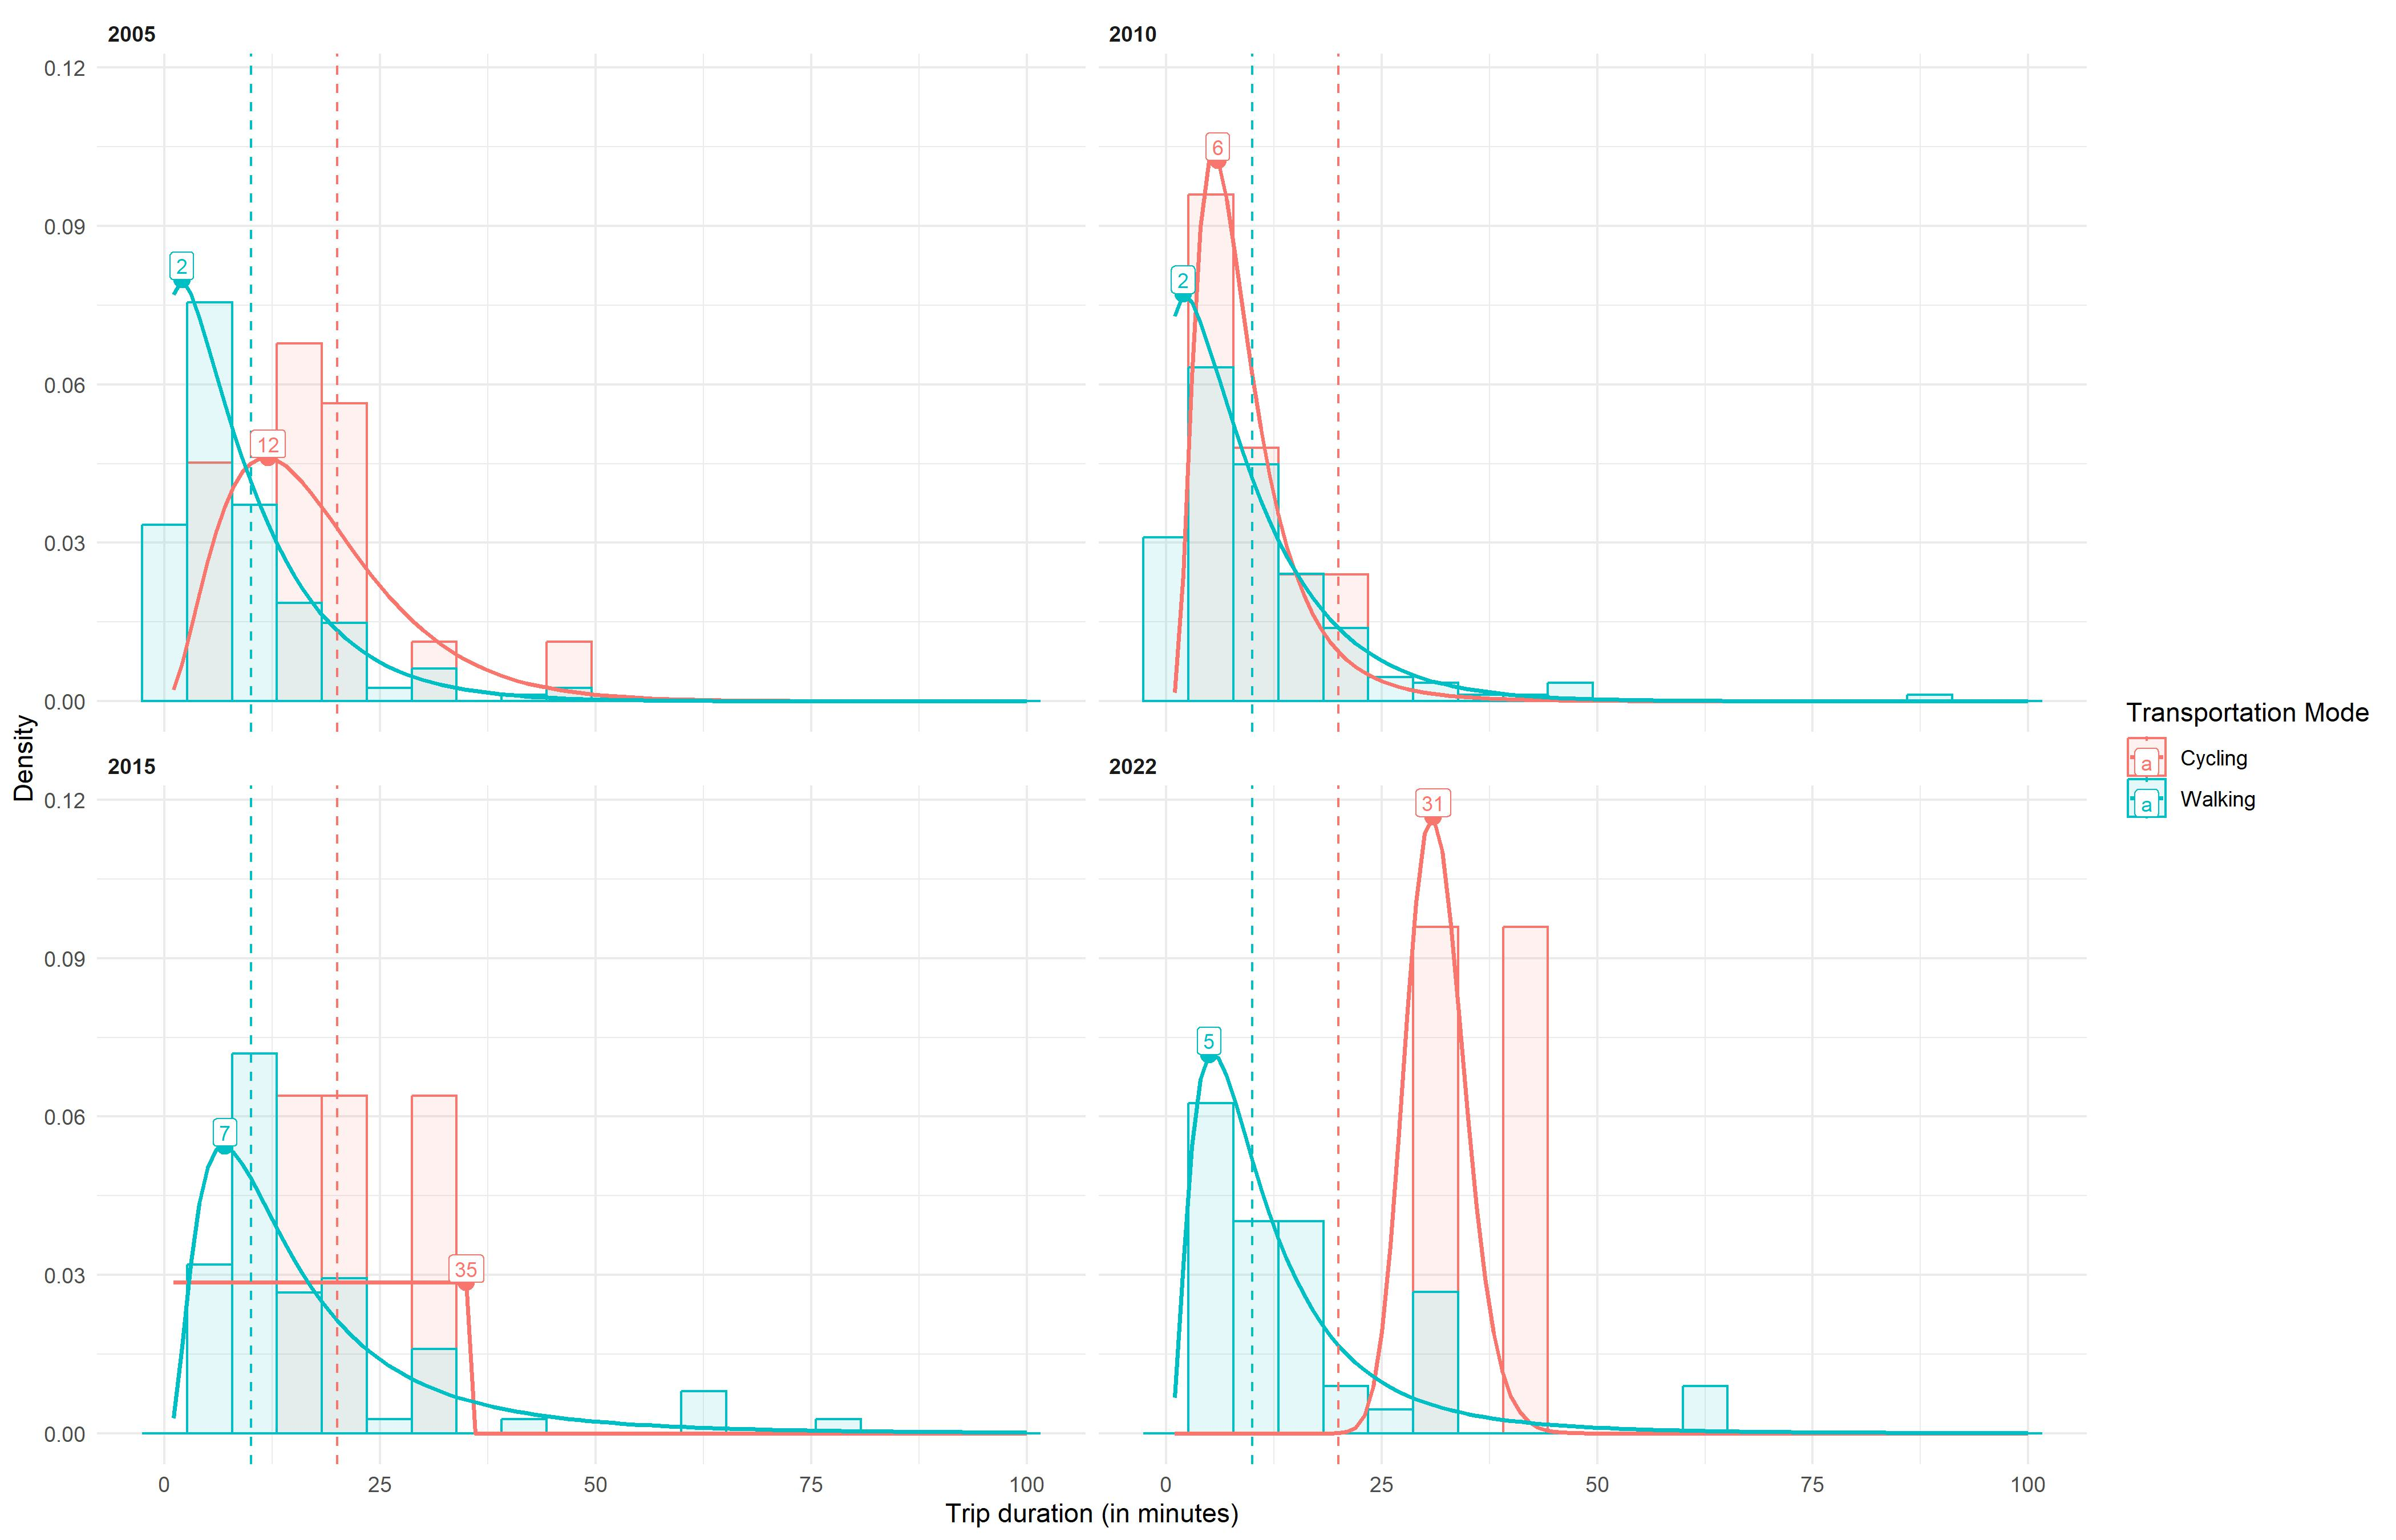
\includegraphics[width=1\linewidth]{figures/impf_Outdoors} 

}

\caption{Empirical data and impedance functions fitted for walking trips with `work or school` as destination.}\label{fig:outdoors-impedance-fig}
\end{figure}

The temporal difference between the decay functions is also evident in
Figure \ref{fig:walking-evolution-fig}, which shows the calibrated
functions for each year of analysis across all destination and transport
mode categories for walking trips. For some locations, the impedance
functions are of the same type and have similar parameters across all
the years analyzed. For example, the ``Cultural venues'', the only
destination present in more than one survey that did not displayed a
statistically significant difference for the walking mode, consistently
uses a gamma function to represent the population's transport behavior
for all the years analyzed. On the other hand, the ``Place of worship''
destination exhibits temporal differences, with distinctly different
peaks and density dispersions, reflecting the variations in the
empirical data shown in Figure \ref{fig:figure-boxplot} and discussed
above.

\begin{figure}

{\centering 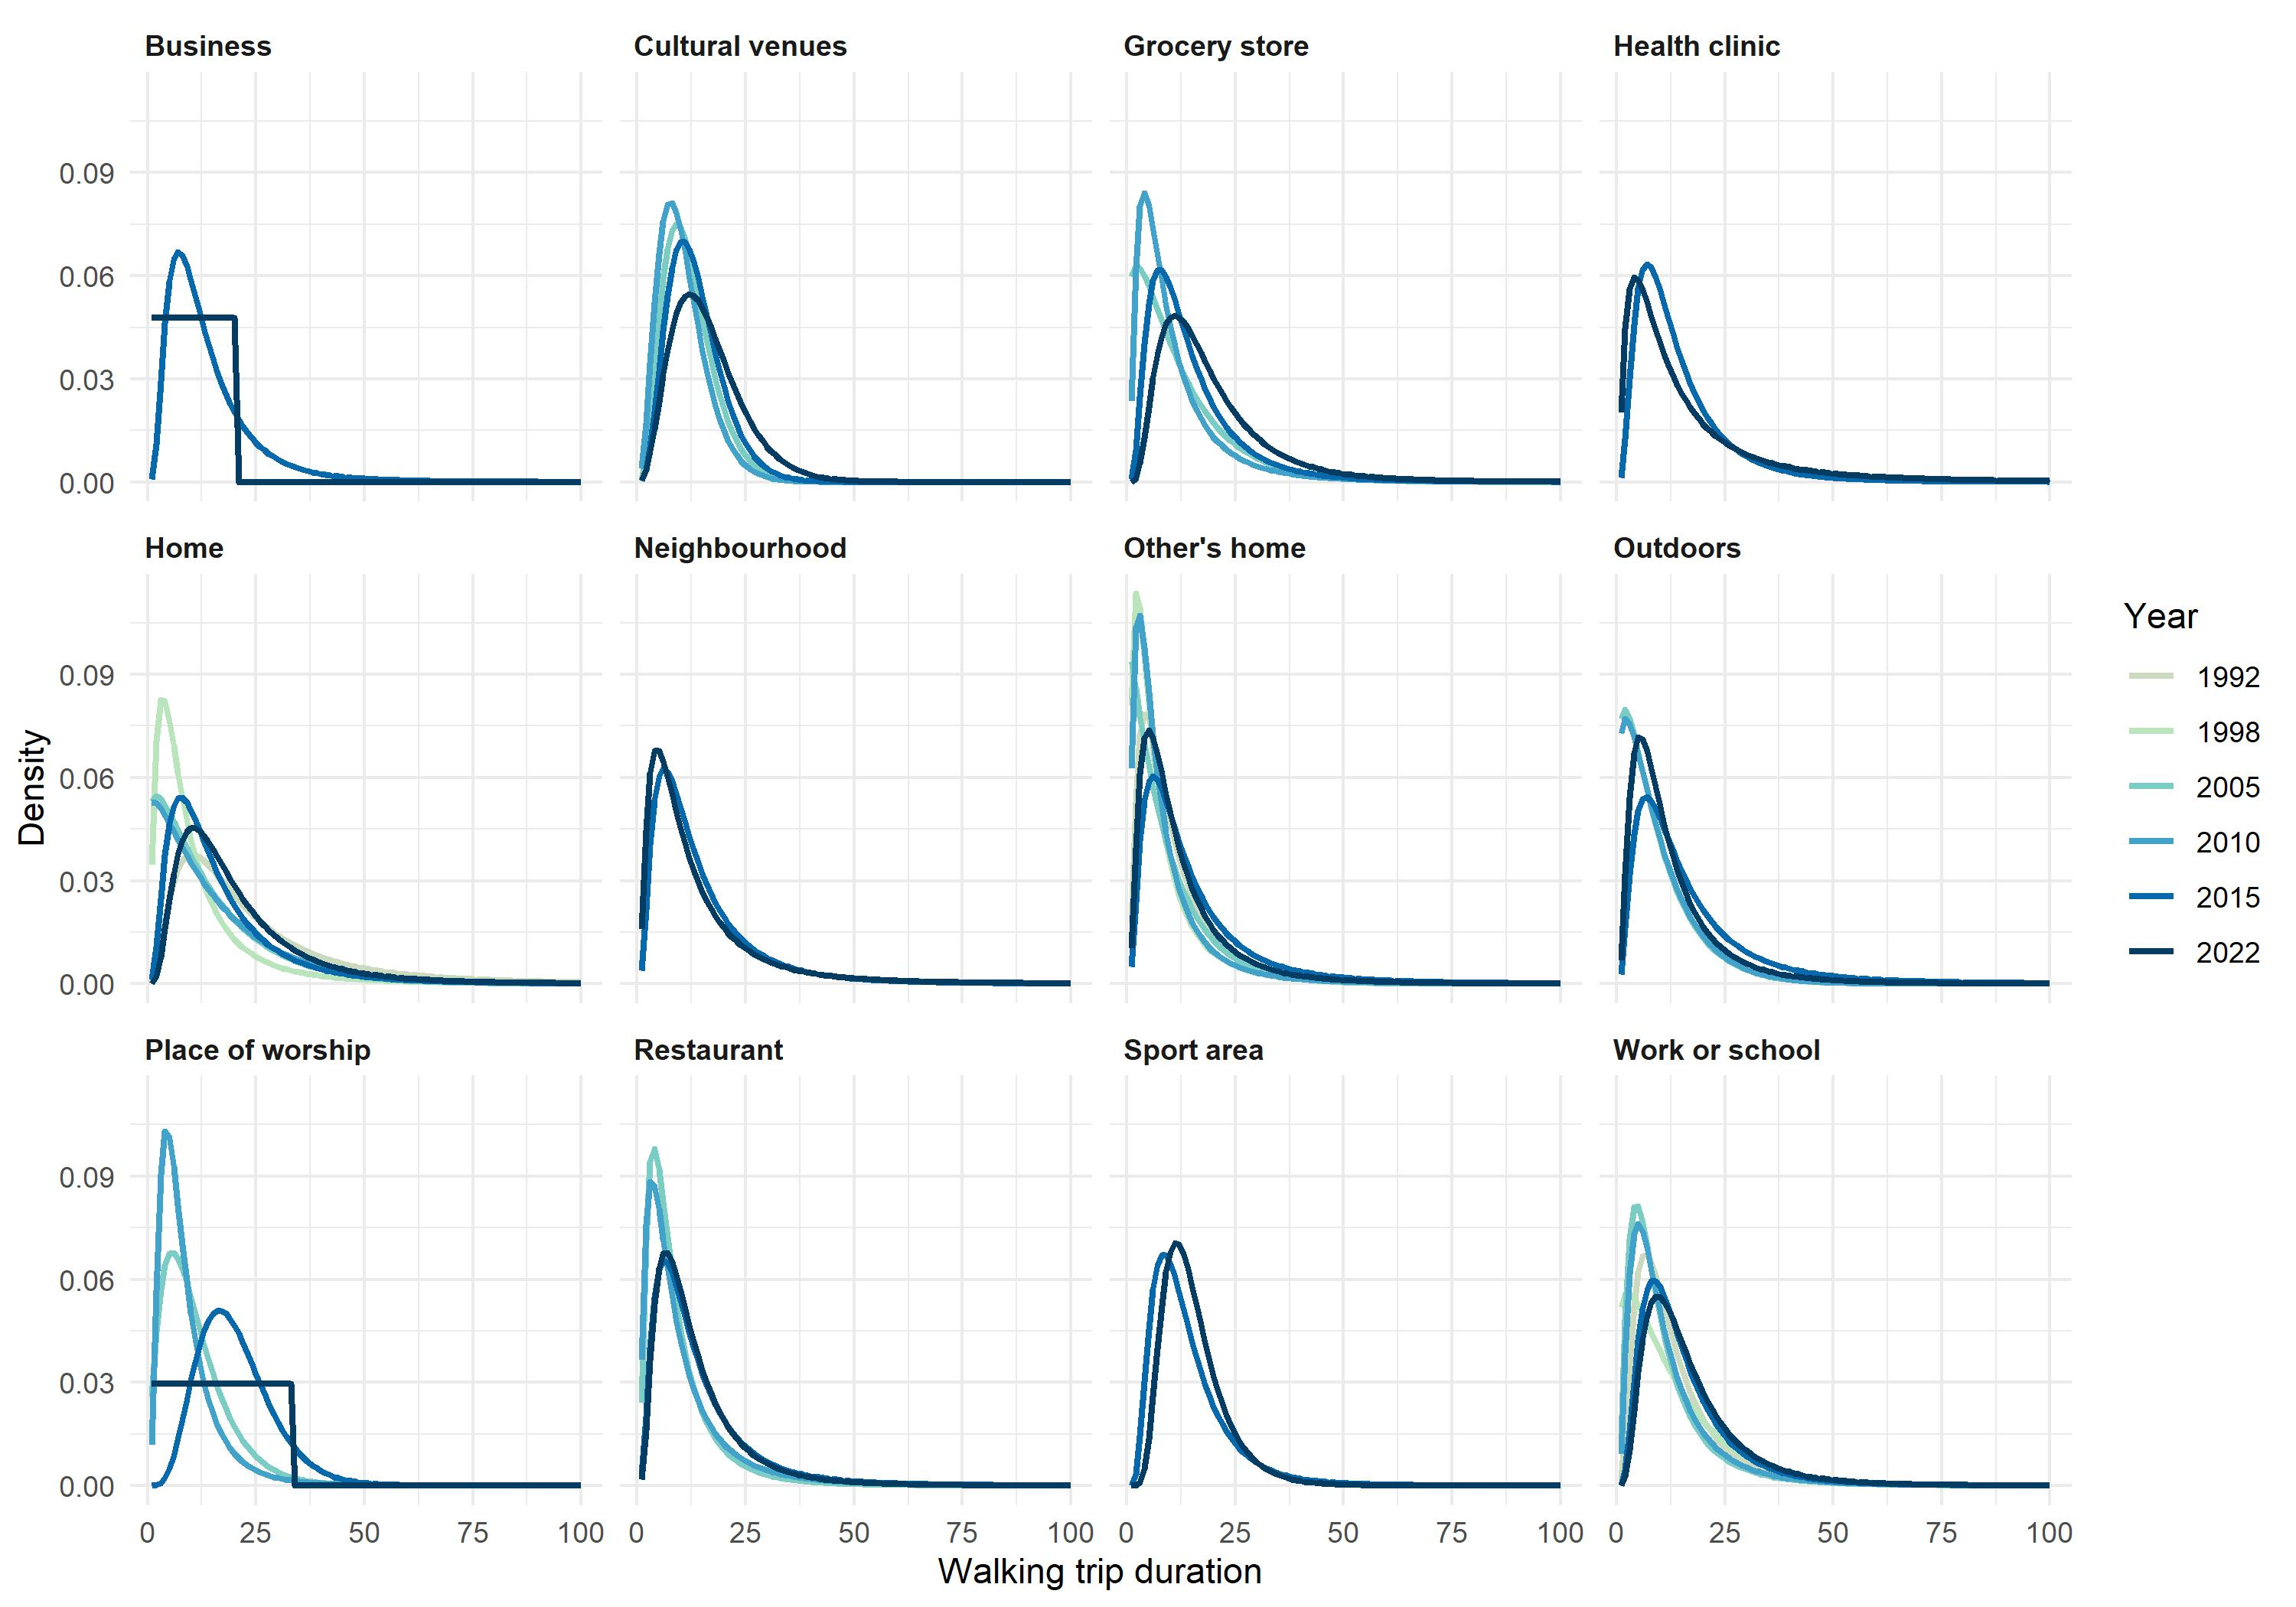
\includegraphics[width=1\linewidth]{figures/walking_temporal_evolution} 

}

\caption{Temporal evolution of walking impedance functions.}\label{fig:walking-evolution-fig}
\end{figure}

Finally, Figures \ref{fig:walking-function-by-year-fig} and
\ref{fig:cycling-function-by-year-fig} present the impedance functions
for different destination categories, grouped by year, for the walking
and cycling modes of transport, respectively.

\begin{figure}

{\centering 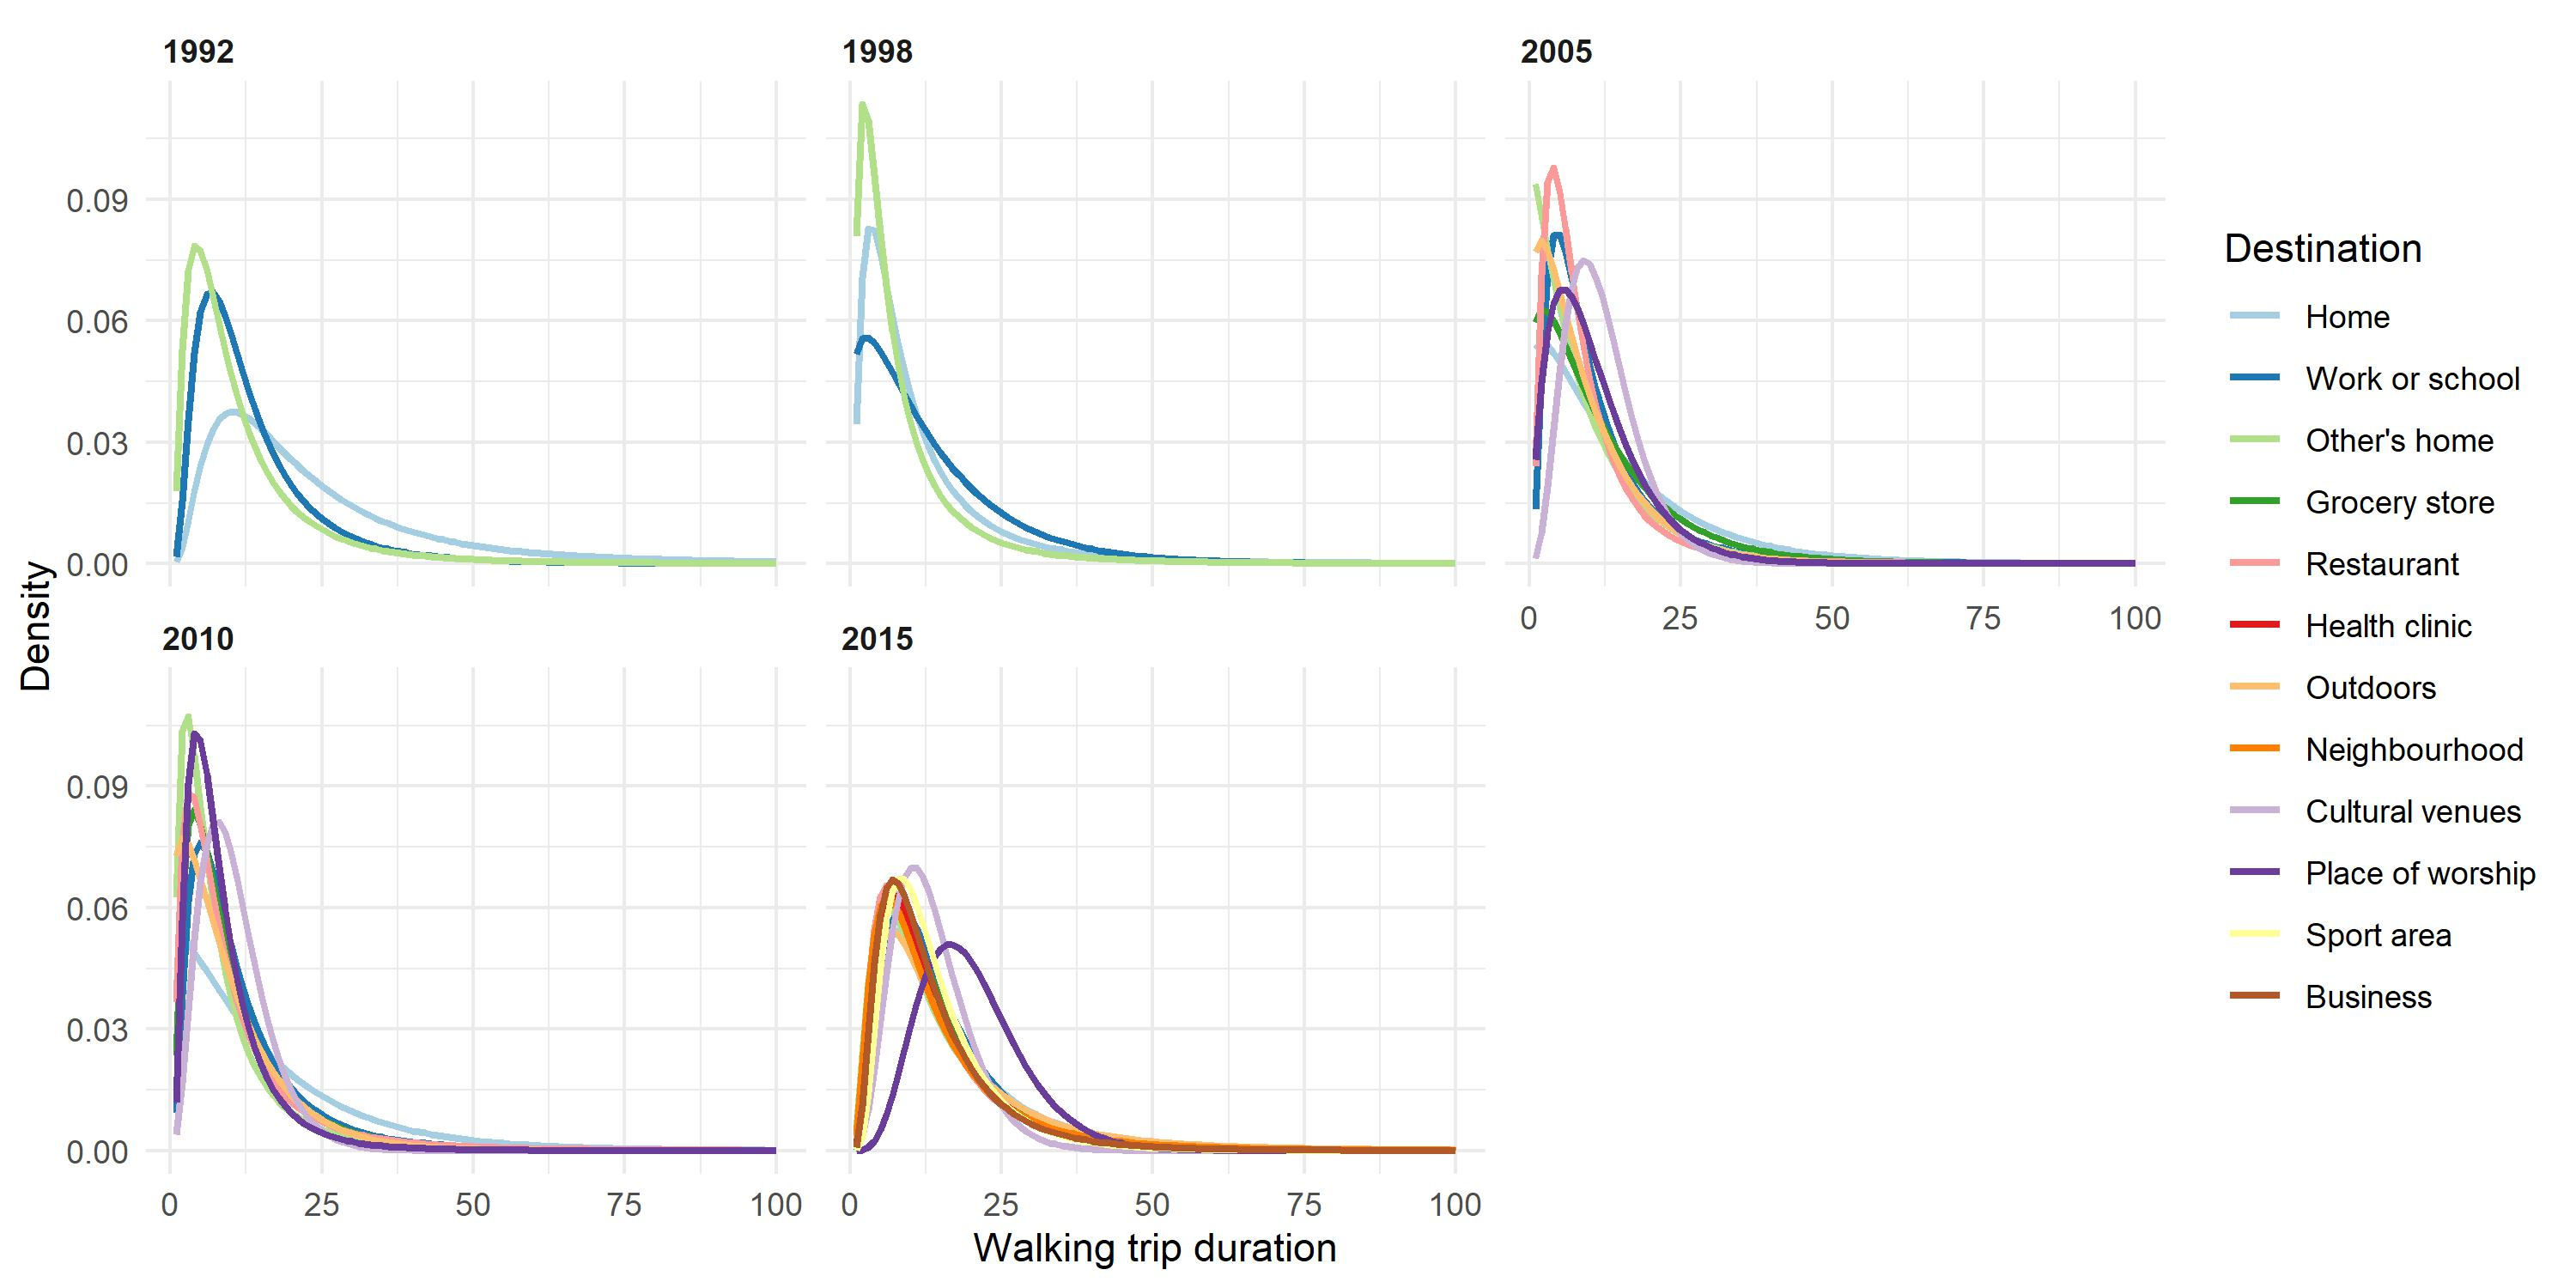
\includegraphics[width=1\linewidth]{figures/walking_functions_by_year} 

}

\caption{Walking functions grouped by year.}\label{fig:walking-function-by-year-fig}
\end{figure}

\begin{figure}

{\centering 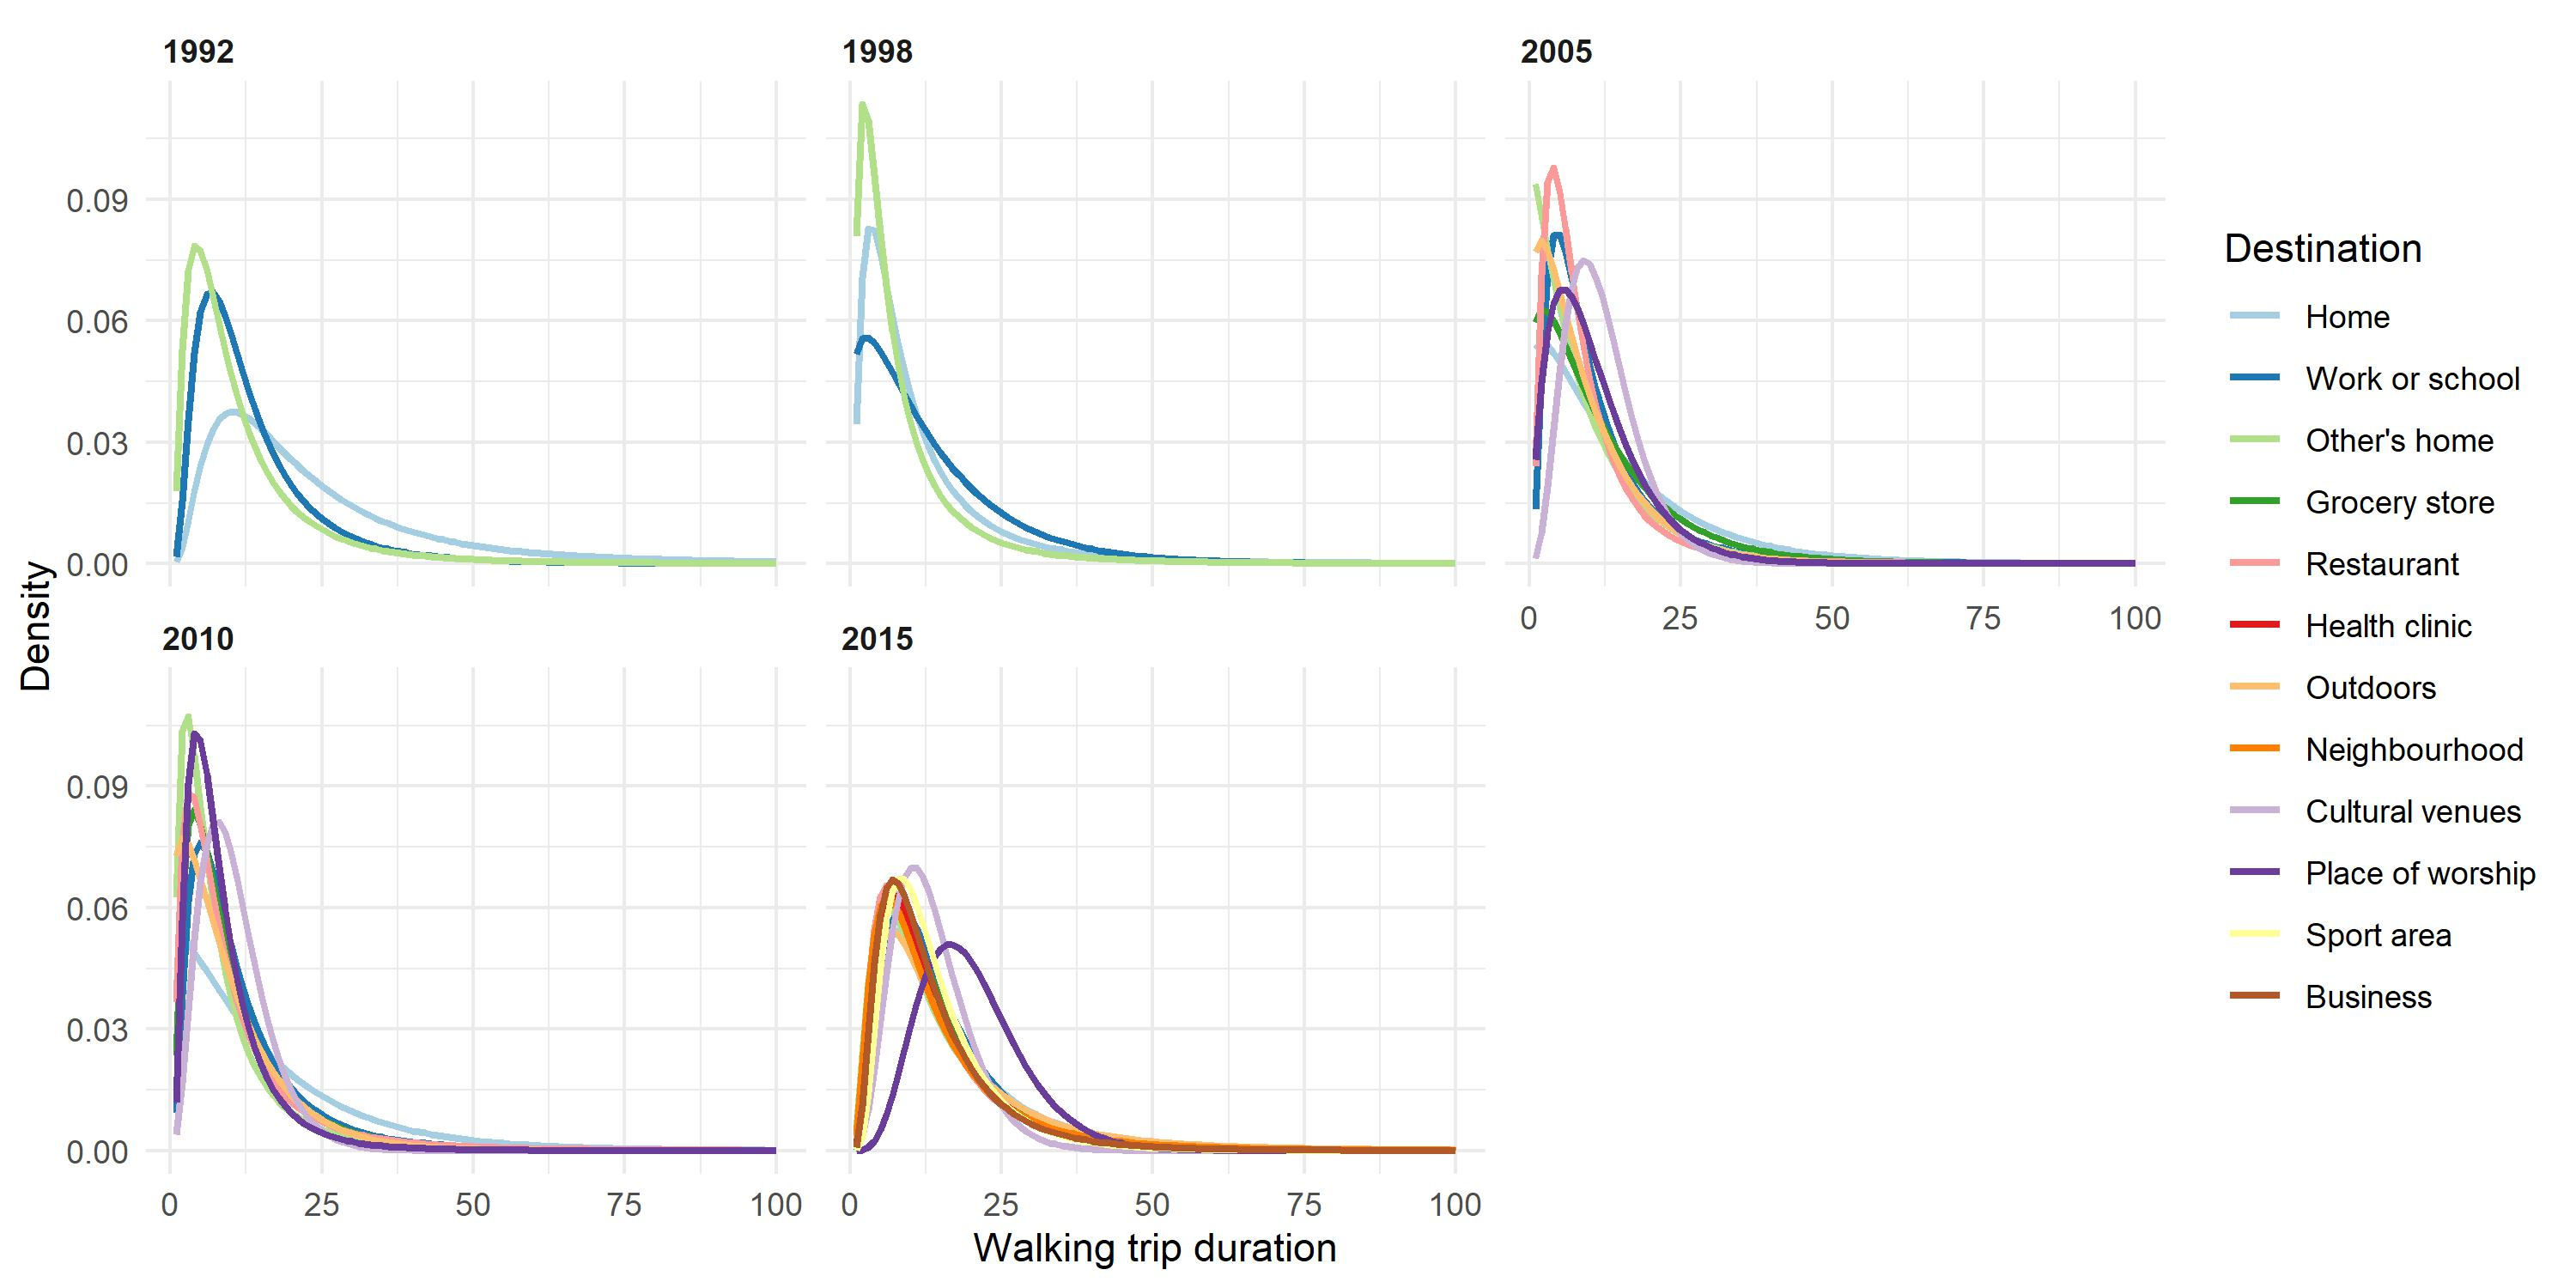
\includegraphics[width=1\linewidth]{figures/cycling_functions_by_year} 

}

\caption{Cycling functions grouped by year.}\label{fig:cycling-function-by-year-fig}
\end{figure}

\section{Summary and conclusion}\label{summary-and-conclusion}

The main objectives of this study were to provide an overview of active
transportation in Canadian metropolitan cities, focusing on primary
origins, destinations, and travel times, and to identify appropriate
impedance functions for active transportation modes across various
destinations and time periods. In this study we perform a direct
application of \texttt{ActiveCA} R package (Dos Santos, Moghadasi, and
Páez, n.d.), analyzing over 12,000 cases of active travel trips that
represented 22,731,111 episodes, from the Time Use cycles of the General
Social Survey (GSS) from 1992 to 2015, covering a twelve different type
of destinations and considering walking and cycling as transportation
modes.

Although the study does not explain the reasons for fluctuations in
travel times over the years, the findings confirmed with statistical
significance, that typical active travel times remained constant for
walking mode, and increased after a dropped since 1998 for cycling mode.
For walking trips, typical travel times remained constant at 10 minutes
since 2005. For cycling trips, the typical travel time fluctuated from
20 minutes in 1992 to 25 minutes in 1998, dropped to 15 minutes in 2005,
dropped again to 10 minutes in 2010, and returned to increase to 20
minutes in 2015. The results also show that, in general, typical travel
times for walking were consistently lower than for cycling.

For walking trips, travel times to `Restaurants' and `Outdoors' rose
from 5 minutes in 2005 to 10 minutes in 2015, while travel to `Places of
worship' increased from 10 minutes in 2005 to 20 minutes in 2015,
marking the highest typical travel time for walking trips. The walking
travel time for `Home' and `Work or school' remained constant at 10
minutes since at least the three last GSS cycles. For cycling trips, the
year of 2015 displayed a trend of increasing travel times for almost all
destinations. This trend is perceptible and statistically significant
for `Grocery store' (rising from 10 to 15 minutes between 2005 and
2015), `Outdoors' (from 15 to 30 minutes during the same period), and
`Restaurant' (from 15 minutes in 2005 to 20 minutes in 2015). `Home'
returned to 20 minutes in 2015 after a drop to 10 minutes in 2010.

For both transportation modes, the destination `Other's home' showed a
decline in the share of trips, reflecting changes in travel behavior
since the technological advances enabled people to maintain contact with
friends and relatives without visiting in person. For walking trips,
findings indicate that `Home' remains the main hub, whether as an origin
or destination. For cycling trips, the combination of `Home' and `Work
or school' accounted for the largest share of trips.

The population share with at least one active trip record ranged from
7.8\% in 1998 (the lowest, 1,892,299 people) to 14.5\% in 2010 (the
peak, 4,084,114 people). In the most recent GSS survey, from 2015,
participation decreased to 11\% (3,265,846 people). Walking trips
dominate active trips. Approximately 84\% of the walking population and
90\% of the cycling population recorded only one trip. The maximum
number of trips recorded by a person was 10 (in 1992, 2005, and 2010)
for the walking population and 4 (in 2005) for the cycling population.
The number of active trips per person in the general population was
close to 0. Among the active population, this value averaged 1.180 trips
per person. A decreasing trend in the number of active episodes per
person was detected, whether analyzed in terms of walking or cycling
episodes.

The study highlights the need to apply specific impedance functions for
different destinations when measuring the cost decay effect in
accessibility analyses. Based on this, we fitted 64 impedance functions
for active transportation over more than 30 years, considering different
types of destinations and transportation modes. The results indicate
that none of the parameterized functions were exponential, suggesting
that the impedance functions commonly used in active accessibility
studies may not accurately capture travel behavior, especially for very
short trips (up to 3 minutes), by giving to shorter trips higher
probability of being made. Destinations with a high number of episodes
were primarily fitted with gamma functions, followed by lognormal
functions, while destinations with fewer episodes (fewer than six) were
fitted with a uniform distribution.

Given similarities in urbanization processes between Canada, the United
States, Australia, and West Europe, these findings may also be
applicable to metropolitan areas in those regions. Finally, this study
contributes to the ongoing discussion on active transportation,
emphasizing its importance in promoting sustainable transportation
planning.

\section*{References}\label{references}
\addcontentsline{toc}{section}{References}

\phantomsection\label{refs}
\begin{CSLReferences}{1}{0}
\bibitem[\citeproctext]{ref-akaike1974}
Akaike, Hirotugu. 1974. {``A New Look at the Statistical Model
Identification.''} \emph{IEEE Transactions on Automatic Control} 19 (6):
716--23. \url{https://doi.org/10.1109/TAC.1974.1100705}.

\bibitem[\citeproctext]{ref-apparicio2008comparing}
Apparicio, Philippe, Mohamed Abdelmajid, Mylene Riva, and Richard
Shearmur. 2008. {``Comparing Alternative Approaches to Measuring the
Geographical Accessibility of Urban Health Services: Distance Types and
Aggregation-Error Issues.''} \emph{International Journal of Health
Geographics} 7 (1): 1--14.

\bibitem[\citeproctext]{ref-arranz2019measuring}
Arranz-Lopez, Aldo, Julio A Soria-Lara, Frank Witlox, and Antonio Paez.
2019. {``Measuring Relative Non-Motorized Accessibility to Retail
Activities.''} \emph{International Journal of Sustainable
Transportation} 13 (9): 639--51.

\bibitem[\citeproctext]{ref-arribas-bel2021}
Arribas-Bel, Dani, Mark Green, Francisco Rowe, and Alex Singleton. 2021.
{``Open Data Products-A Framework for Creating Valuable Analysis Ready
Data.''} \emph{Journal of Geographical Systems} 23 (4): 497--514.
\url{https://doi.org/10.1007/s10109-021-00363-5}.

\bibitem[\citeproctext]{ref-bhat2002development}
Bhat, Chandra, Susan Handy, Kara Kockelman, Hani Mahmassani, Anand
Gopal, Issam Srour, and Lisa Weston. 2002. {``Development of an Urban
Accessibility Index: Formulations, Aggregation, and Application.''}
\emph{Work} 4938 (4).

\bibitem[\citeproctext]{ref-statisticscanada2022}
Canada, Statistics. 2022. {``Time Use Survey.''} Ottawa.
\url{https://www23.statcan.gc.ca/imdb/p2SV.pl?Function=getSurvey&amp;SDDS=4503}.

\bibitem[\citeproctext]{ref-carrothers1956historical}
Carrothers, Gerald AP. 1956. {``An Historical Review of the Gravity and
Potential Concepts of Human Interaction.''} \emph{Journal of the
American Institute of Planners} 22 (2): 94--102.

\bibitem[\citeproctext]{ref-cascetta2013new}
Cascetta, Ennio, Armando Carteni, and Marcello Montanino. 2013. {``A New
Measure of Accessibility Based on Perceived Opportunities.''}
\emph{Procedia-Social and Behavioral Sciences} 87: 117--32.

\bibitem[\citeproctext]{ref-church2003measuring}
Church, Richard L, and James R Marston. 2003. {``Measuring Accessibility
for People with a Disability.''} \emph{Geographical Analysis} 35 (1):
83--96.

\bibitem[\citeproctext]{ref-clifton2001evaluating}
Clifton, KELLY J, and SL Handy. 2001. {``Evaluating Neighborhood
Accessibility: Possibilities and Practicalities.''} \emph{Journal of
Transportation and Statistics} 4 (2-3): 67.

\bibitem[\citeproctext]{ref-currie2010quantifying}
Currie, Graham. 2010. {``Quantifying Spatial Gaps in Public Transport
Supply Based on Social Needs.''} \emph{Journal of Transport Geography}
18 (1): 31--41.

\bibitem[\citeproctext]{ref-de2009exponential}
De Vries, Jacob J, Peter Nijkamp, and Piet Rietveld. 2009.
{``Exponential or Power Distance-Decay for Commuting? An Alternative
Specification.''} \emph{Environment and Planning A} 41 (2): 461--80.

\bibitem[\citeproctext]{ref-delignette2015fitdistrplus}
Delignette-Muller, Marie Laure, and Christophe Dutang. 2015.
{``Fitdistrplus: An r Package for Fitting Distributions.''}
\emph{Journal of Statistical Software} 64: 1--34.

\bibitem[\citeproctext]{ref-dossantos2024ActiveCA}
Dos Santos, Bruno Dias, Mahdis Moghadasi, and Antonio Páez. n.d.
{``ActiveCA.''}

\bibitem[\citeproctext]{ref-dunn2023}
Dunn, William L., and J. Kenneth Shultis. 2023. {``Appendix a - Some
Common Probability Distributions.''} In, edited by William L. Dunn and
J. Kenneth Shultis, 447--95. Elsevier.
\url{https://doi.org/10.1016/B978-0-12-819739-4.00019-6}.

\bibitem[\citeproctext]{ref-eldridge1991warped}
Eldridge, J Douglas, and John Paul Jones III. 1991. {``Warped Space: A
Geography of Distance Decay.''} \emph{The Professional Geographer} 43
(4): 500--511.

\bibitem[\citeproctext]{ref-fotheringham1981spatial}
Fotheringham, A Stewart. 1981. {``Spatial Structure and Distance-Decay
Parameters.''} \emph{Annals of the Association of American Geographers}
71 (3): 425--36.

\bibitem[\citeproctext]{ref-fotheringham1989spatial}
Fotheringham, A Stewart, and Morton E O'Kelly. 1989. \emph{Spatial
Interaction Models: Formulations and Applications}. Vol. 1. Kluwer
Academic Publishers Dordrecht.

\bibitem[\citeproctext]{ref-frank2001built}
Frank, Lawrence D, and Peter O Engelke. 2001. {``The Built Environment
and Human Activity Patterns: Exploring the Impacts of Urban Form on
Public Health.''} \emph{Journal of Planning Literature} 16 (2): 202--18.

\bibitem[\citeproctext]{ref-frank2005linking}
Frank, Lawrence D, Thomas L Schmid, James F Sallis, James Chapman, and
Brian E Saelens. 2005. {``Linking Objectively Measured Physical Activity
with Objectively Measured Urban Form: Findings from SMARTRAQ.''}
\emph{American Journal of Preventive Medicine} 28 (2): 117--25.

\bibitem[\citeproctext]{ref-geurs2001accessibility}
Geurs, Karst T, and Jan R Ritsema van Eck. 2001. {``Accessibility
Measures: Review and Applications. Evaluation of Accessibility Impacts
of Land-Use Transportation Scenarios, and Related Social and Economic
Impact.''} \emph{RIVM Rapport 408505006}.

\bibitem[\citeproctext]{ref-geurs2004}
Geurs, Karst T, and Bert Van Wee. 2004. {``Accessibility Evaluation of
Land-Use and Transport Strategies: Review and Research Directions.''}
\emph{Journal of Transport Geography} 12 (2): 127--40.

\bibitem[\citeproctext]{ref-grengs2015nonwork}
Grengs, Joe. 2015. {``Nonwork Accessibility as a Social Equity
Indicator.''} \emph{International Journal of Sustainable Transportation}
9 (1): 1--14.

\bibitem[\citeproctext]{ref-gutierrez1996european}
Gutierrez, Javier, Rafael Gonzalez, and Gabriel Gomez. 1996. {``The
European High-Speed Train Network: Predicted Effects on Accessibility
Patterns.''} \emph{Journal of Transport Geography} 4 (4): 227--38.

\bibitem[\citeproctext]{ref-handy1993regional}
Handy, Susan. 1993. {``Regional Versus Local Accessibility: Implications
for Nonwork Travel.''}

\bibitem[\citeproctext]{ref-handy1997measuring}
Handy, Susan L, and Debbie A Niemeier. 1997. {``Measuring Accessibility:
An Exploration of Issues and Alternatives.''} \emph{Environment and
Planning A} 29 (7): 1175--94.

\bibitem[\citeproctext]{ref-hansen1959accessibility}
Hansen, Walter G. 1959. {``How Accessibility Shapes Land Use.''}
\emph{Journal of the American Institute of Planners} 25 (2): 73--76.

\bibitem[\citeproctext]{ref-hino2014built}
Hino, Adriano AF, Rodrigo S Reis, Olga L Sarmiento, Diana C Parra, and
Ross C Brownson. 2014. {``Built Environment and Physical Activity for
Transportation in Adults from Curitiba, Brazil.''} \emph{Journal of
Urban Health} 91: 446--62.

\bibitem[\citeproctext]{ref-hsiao1997use}
Hsiao, Shirley, Jian Lu, James Sterling, and Matthew Weatherford. 1997.
{``Use of Geographic Information System for Analysis of Transit
Pedestrian Access.''} \emph{Transportation Research Record} 1604 (1):
50--59.

\bibitem[\citeproctext]{ref-hull2012accessibility}
Hull, Angela, Cecilia Silva, and Luca Bertolini. 2012.
\emph{Accessibility Instruments for Planning Practice}. Cost Office
Brussels.

\bibitem[\citeproctext]{ref-iacono2010}
Iacono, Michael, Kevin J Krizek, and Ahmed El-Geneidy. 2010.
{``Measuring Non-Motorized Accessibility: Issues, Alternatives, and
Execution.''} \emph{Journal of Transport Geography} 18 (1): 133--40.

\bibitem[\citeproctext]{ref-iacono2008access}
Iacono, Michael, Kevin Krizek, and Ahmed M El-Geneidy. 2008. {``Access
to Destinations: How Close Is Close Enough? Estimating Accurate Distance
Decay Functions for Multiple Modes and Different Purposes.''}

\bibitem[\citeproctext]{ref-itf2017linking}
ITF. 2017. \emph{Linking People and Places: New Ways of Understanding
Spatial Access in Cities}. OECD Publishing.

\bibitem[\citeproctext]{ref-kanafani1983transportation}
Kanafani, Adib. 1983. {``Transportation Demand Analysis.''}

\bibitem[\citeproctext]{ref-koenig1980indicators}
Koenig, Jean-Gerard. 1980. {``Indicators of Urban Accessibility: Theory
and Application.''} \emph{Transportation} 9 (2): 145--72.

\bibitem[\citeproctext]{ref-krizek2005perspectives}
Krizek, Kevin J. 2005. {``Perspectives on Accessibility and Travel.''}
In \emph{Access to Destinations}, 109--30. Emerald Group Publishing
Limited.

\bibitem[\citeproctext]{ref-kwan1998space}
Kwan, Mei-Po. 1998. {``Space-Time and Integral Measures of Individual
Accessibility: A Comparative Analysis Using a Point-Based Framework.''}
\emph{Geographical Analysis} 30 (3): 191--216.

\bibitem[\citeproctext]{ref-kwan2003recent}
Kwan, Mei-Po, Alan T Murray, Morton E OKelly, and Michael Tiefelsdorf.
2003. {``Recent Advances in Accessibility Research: Representation,
Methodology and Applications.''} \emph{Journal of Geographical Systems}
5: 129--38.

\bibitem[\citeproctext]{ref-lamiquiz2015effects}
Lamiquiz, Patxi J, and Jorge Lopez-Dominguez. 2015. {``Effects of Built
Environment on Walking at the Neighbourhood Scale. A New Role for Street
Networks by Modelling Their Configurational Accessibility?''}
\emph{Transportation Research Part A: Policy and Practice} 74: 148--63.

\bibitem[\citeproctext]{ref-larsen2010beyond}
Larsen, Jacob, Ahmed El-Geneidy, and Farhana Yasmin. 2010. {``Beyond the
Quarter Mile: Re-Examining Travel Distances by Active Transportation.''}
\emph{Canadian Journal of Urban Research} 19 (1): 70--88.

\bibitem[\citeproctext]{ref-levinson2005access}
Levinson, David M, and Kevin J Krizek. 2005. \emph{Access to
Destinations}. Elsevier Publishers.

\bibitem[\citeproctext]{ref-li2020approach}
Li, Aoyong, Yizhe Huang, and Kay W Axhausen. 2020. {``An Approach to
Imputing Destination Activities for Inclusion in Measures of Bicycle
Accessibility.''} \emph{Journal of Transport Geography} 82: 102566.

\bibitem[\citeproctext]{ref-lowry2012using}
Lowry, M, Daniel Callister, M Gresham, and B Moore. 2012. {``Using
Bicycle Level of Service to Assess Community-Wide Bikeability.''} In
\emph{91st Annual Meeting of the Transportation Research Board,
Washington, DC: Transportation Research Board}.

\bibitem[\citeproctext]{ref-luoma1993threshold}
Luoma, Martti, Kauko Mikkonen, and Mauri Palomaki. 1993. {``The
Threshold Gravity Model and Transport Geography: How Transport
Development Influences the Distance-Decay Parameter of the Gravity
Model.''} \emph{Journal of Transport Geography} 1 (4): 240--47.

\bibitem[\citeproctext]{ref-meyer1984urban}
Meyer, Michael D, and Eric J Miller. 1984. {``Urban Transportation
Planning: A Decision-Oriented Approach.''}

\bibitem[\citeproctext]{ref-mikkonen1999parameters}
Mikkonen, Kauko, and Martti Luoma. 1999. {``The Parameters of the
Gravity Model Are Changing--How and Why?''} \emph{Journal of Transport
Geography} 7 (4): 277--83.

\bibitem[\citeproctext]{ref-miller2005place}
Miller, Harvey J. 2005. {``Place-Based Versus People-Based
Accessibility.''} In \emph{Access to Destinations}, 63--89. Emerald
Group Publishing Limited.

\bibitem[\citeproctext]{ref-millward2013active}
Millward, Hugh, Jamie Spinney, and Darren Scott. 2013.
{``Active-Transport Walking Behavior: Destinations, Durations,
Distances.''} \emph{Journal of Transport Geography} 28: 101--10.

\bibitem[\citeproctext]{ref-moreno2021}
Moreno, Carlos, Zaheer Allam, Didier Chabaud, Catherine Gall, and
Florent Pratlong. 2021. {``Introducing the {``}15-Minute City{''}:
Sustainability, Resilience and Place Identity in Future Post-Pandemic
Cities.''} \emph{Smart Cities} 4 (1): 93--111.
\url{https://doi.org/10.3390/smartcities4010006}.

\bibitem[\citeproctext]{ref-nassir2016utility}
Nassir, Neema, Mark Hickman, Ali Malekzadeh, and Elnaz Irannezhad. 2016.
{``A Utility-Based Travel Impedance Measure for Public Transit Network
Accessibility.''} \emph{Transportation Research Part A: Policy and
Practice} 88: 26--39.

\bibitem[\citeproctext]{ref-osth2016new}
Osth, John, Johan Lyhagen, and Aura Reggiani. 2016. {``A New Way of
Determining Distance Decay Parameters in Spatial Interaction Models with
Application to Job Accessibility Analysis in Sweden.''} \emph{European
Journal of Transport and Infrastructure Research} 16 (2).

\bibitem[\citeproctext]{ref-puxe1ez2021}
Páez, Antonio. 2021. {``Open Spatial Sciences: An Introduction.''}
\emph{Journal of Geographical Systems} 23 (4): 467--76.
\url{https://doi.org/10.1007/s10109-021-00364-4}.

\bibitem[\citeproctext]{ref-puxe1ez2012}
Páez, Antonio, Darren M. Scott, and Catherine Morency. 2012.
{``Measuring Accessibility: Positive and Normative Implementations of
Various Accessibility Indicators.''} \emph{Journal of Transport
Geography}, Special section on accessibility and socio-economic
activities: Methodological and empirical aspects, 25 (November):
141--53. \url{https://doi.org/10.1016/j.jtrangeo.2012.03.016}.

\bibitem[\citeproctext]{ref-papa2012gravity}
Papa, Enrica, and Pierluigi Coppola. 2012. {``Gravity-Based
Accessibility Measures for Integrated Transport-Land Use Planning
(GraBAM).''} \emph{Accessibility Instruments for Planning Practice} 117:
124.

\bibitem[\citeproctext]{ref-pereira2023}
Pereira, Rafael H. M., and Daniel Herszenhut. 2023. {``Accessibility
measures.''} In. Rio de Janeiro.
\url{https://doi.org/10.38116/9786556350653}.

\bibitem[\citeproctext]{ref-pereira2017}
Pereira, Rafael H. M., Tim Schwanen, and David Banister. 2017.
{``Distributive Justice and Equity in Transportation.''} \emph{Transport
Reviews} 37 (2): 170--91.
\url{https://doi.org/10.1080/01441647.2016.1257660}.

\bibitem[\citeproctext]{ref-pirie1979measuring}
Pirie, Gordon H. 1979. {``Measuring Accessibility: A Review and
Proposal.''} \emph{Environment and Planning A} 11 (3): 299--312.

\bibitem[\citeproctext]{ref-prins2014many}
Prins, Richard G, Frank Pierik, Astrid Etman, Reinier P Sterkenburg,
Carlijn BM Kamphuis, and FJ Van Lenthe. 2014. {``How Many Walking and
Cycling Trips Made by Elderly Are Beyond Commonly Used Buffer Sizes:
Results from a GPS Study.''} \emph{Health \& Place} 27: 127--33.

\bibitem[\citeproctext]{ref-reggiani2011accessibility}
Reggiani, Aura, Pietro Bucci, and Giovanni Russo. 2011. {``Accessibility
and Impedance Forms: Empirical Applications to the German Commuting
Network.''} \emph{International Regional Science Review} 34 (2):
230--52.

\bibitem[\citeproctext]{ref-saghapour2017measuring}
Saghapour, Tayebeh, Sara Moridpour, and Russell G Thompson. 2017.
{``Measuring Cycling Accessibility in Metropolitan Areas.''}
\emph{International Journal of Sustainable Transportation} 11 (5):
381--94.

\bibitem[\citeproctext]{ref-sallis2004active}
Sallis, James F, Lawrence D Frank, Brian E Saelens, and M Katherine
Kraft. 2004. {``Active Transportation and Physical Activity:
Opportunities for Collaboration on Transportation and Public Health
Research.''} \emph{Transportation Research Part A: Policy and Practice}
38 (4): 249--68.

\bibitem[\citeproctext]{ref-signorino2011gravity}
Signorino, Guido, Roberto Pasetto, Elisa Gatto, Massimo Mucciardi,
Marina La Rocca, and Pierpaolo Mudu. 2011. {``Gravity Models to Classify
Commuting Vs. Resident Workers. An Application to the Analysis of
Residential Risk in a Contaminated Area.''} \emph{International Journal
of Health Geographics} 10 (1): 1--10.

\bibitem[\citeproctext]{ref-skov2001estimation}
Skov-Petersen, Hans. 2001. {``Estimation of Distance-Decay Parameters:
GIS-Based Indicators of Recreational Accessibility.''} In
\emph{ScanGIS}, 237--58.

\bibitem[\citeproctext]{ref-soukhov2024}
Soukhov, Anastasia, and Antonio Paez. 2024. {``Accessibility Analysis
for Planning Applications.''}
\url{https://github.com/soukhova/MJ-Accessibility-Blogs}.

\bibitem[\citeproctext]{ref-sun2012measuring}
Sun, Guibo, Hui Lin, and Rongrong Li. 2012. {``Measuring the Influence
of Built Environment on Walking Behavior: An Accessibility Approach.''}
In \emph{Geographic Information Science: 7th International Conference,
GIScience 2012, Columbus, OH, USA, September 18-21, 2012. Proceedings
7}, 187--97. Springer.

\bibitem[\citeproctext]{ref-taylor1975distance}
Taylor, Peter. 1975. {``Distance Decay Models in Spatial
Interactions.''} \emph{(No Title)}.

\bibitem[\citeproctext]{ref-untermann1984accommodating}
Untermann, Richard K. 1984. {``Accommodating the Pedestrian: Adapting
Towns and Neighbourhoods for Walking and Bicycling.''}

\bibitem[\citeproctext]{ref-vale2017influence}
Vale, David S, and Mauro Pereira. 2017. {``The Influence of the
Impedance Function on Gravity-Based Pedestrian Accessibility Measures: A
Comparative Analysis.''} \emph{Environment and Planning B: Urban
Analytics and City Science} 44 (4): 740--63.

\bibitem[\citeproctext]{ref-vandenbulcke2009mapping}
Vandenbulcke, Gregory, Therese Steenberghen, and Isabelle Thomas. 2009.
{``Mapping Accessibility in Belgium: A Tool for Land-Use and Transport
Planning?''} \emph{Journal of Transport Geography} 17 (1): 39--53.

\bibitem[\citeproctext]{ref-vasconcelos2012evaluation}
Vasconcelos, Ana S, and Tiago L Farias. 2012. {``Evaluation of Urban
Accessibility Indicators Based on Internal and External Environmental
Costs.''} \emph{Transportation Research Part D: Transport and
Environment} 17 (6): 433--41.

\bibitem[\citeproctext]{ref-vega2012using}
Vega, Amaya. 2012. {``Using Place Rank to Measure Sustainable
Accessibility.''} \emph{Journal of Transport Geography} 24: 411--18.

\bibitem[\citeproctext]{ref-wu2019measuring}
Wu, Xueying, Yi Lu, Yaoyu Lin, and Yiyang Yang. 2019. {``Measuring the
Destination Accessibility of Cycling Transfer Trips in Metro Station
Areas: A Big Data Approach.''} \emph{International Journal of
Environmental Research and Public Health} 16 (15): 2641.

\bibitem[\citeproctext]{ref-yang2012walking}
Yang, Yong, and Ana V Diez-Roux. 2012. {``Walking Distance by Trip
Purpose and Population Subgroups.''} \emph{American Journal of
Preventive Medicine} 43 (1): 11--19.

\bibitem[\citeproctext]{ref-zhao2003forecasting}
Zhao, Fang, Lee-Fang Chow, Min-Tang Li, Ike Ubaka, and Albert Gan. 2003.
{``Forecasting Transit Walk Accessibility: Regression Model Alternative
to Buffer Method.''} \emph{Transportation Research Record} 1835 (1):
34--41.

\end{CSLReferences}


\end{document}
